\documentclass[letterpaper, 12pt, notitlepage]{report}
\usepackage[plainpages=false, colorlinks, urlcolor=black, citecolor=black,
	linkcolor=black]{hyperref}
\usepackage{graphicx}

%A LaTeX package which provides macros for the graphical
%representation of the keys on a computer keyboard.
\usepackage{keystroke}

%http://ctan.dcc.uchile.cl/help/Catalogue/entries/floatrow.html
%\usepackage{floatrow}

\usepackage{longtable}

\usepackage[utf8]{inputenc}
\usepackage{txfonts}
\usepackage{listings}
\usepackage{multirow}
\usepackage{float}
\usepackage[polutonikogreek,english,spanish]{babel}
\usepackage{epsfig}
\usepackage{sty/utfsm_tesis}

%Include Table of Contents as the first entry in TOC
\usepackage{sty/xtocinc}
\usepackage[nottoc]{tocbibind}

%\usepackage[dvips]{epsfig}
%\usepackage{psfig}

\usepackage{caption}
\usepackage{subcaption}

%% Margenes segun Normas
%% Ancho Legal 21,59cm /  8,5in
%% Alto  Legal 33,02cm / 13,0in
%\paperheight    27.81cm % alto letter
%\paperwidth     21.59cm % ancho
%\hoffset        -1.0in % Seteo a 0 el margen izquierdo
%\voffset        -1.0in % Seteo a 0 el margen superior
%\oddsidemargin  3.80cm % Margen izquierdo (pag. impar)
%% \evensidemargin 2.55cm % Margen izquierdo (pag. par) Acrobat Winkk
%\evensidemargin 2.59cm % Margen izquierdo (pag. par)
%\topmargin      1.00cm % Margen superior
%\headheight     5.00mm % Ancho encabezado
%\headsep        8.00mm % Separacion encabezado-cuerpo
%\textheight     23.5cm % Alto cuerpo
%\textwidth      15.2cm % Ancho cuerpo
%\footskip       1.30cm % Separacion piepag-cuerpo
\parindent      0em
\parskip        2ex

% Fuzz -------------------------------------------------------------------
\hfuzz2pt

% \oddsidemargin	 0cm	% Ancho Legal 21,59cm
% \evensidemargin 0.5cm	% Alto	Legal 35,56cm
% \textwidth	 16.5cm
% \topmargin	  -1.5cm
% \textheight	 22cm

\newlength{\defbaselineskip}
\setlength{\defbaselineskip}{\baselineskip}

\newcommand{\setlinespacing}[1]%
	   {\setlength{\baselineskip}{#1 \defbaselineskip}}
\newcommand{\doublespacing}{\setlength{\baselineskip}%
			   {1.3 \defbaselineskip}}
\newcommand{\singlespacing}{\setlength{\baselineskip}{\defbaselineskip}}

\lstloadlanguages{C++, sh, IDL, make}
\lstset{basicstyle=\small\sffamily, commentstyle=\slshape,
        numbers=left, numberstyle=\tiny, numbersep=10pt,
        extendedchars, frame=lines,
        floatplacement=ht, captionpos=b,
        defaultdialect=[CORBA]IDL}



%descomentar para poner fecha distinta a fecha de compilacion
\copyrightyear{2017} \submitdate{Octubre 2017}
\convocation{Octubre}{2017}

\title{Algoritmo para el cálculo de fragmentos de proteínas en los organismos secuenciados}
\author{Felipe Nicolás Araya Barrera}

\begin{document}

\selectlanguage{spanish}

\profguia{Lioubov Dombrovskaia}
\profcorr{Diego Arroyuelo Billiardi}

% Archivo de Agradecimientos
\ack{include/acknowledgements}

% Incluir Resumen
\resumenesp{include/resumen}

% Incluir Abstract
\resumening{include/abstract}

% Incluir Abreviaciones
\abreviaciones{include/glossary}

\beforepreface
\afterpreface

%\numberwithin{equation}{chapter}

% Incluir introduccion
\chapter*{Introducci\'on}
\addcontentsline{toc}{chapter}{Introducci\'on}

\section*{Motivación}

Para el actual documento, las razones que motivaron al alumno presente a realizar la investigación de su tesis son la de comenzar a 
entrar en una rama que en los últimos años ha tomado bastante importancia en la informática, conocida como la {\textit{Bioinformática}} \cite{bioinformatica}, la cual aplica las tecnologías computacionales contemporáneas a datos biológicos que pueden pertenecer a estructuras como ADN, proteínas, entre otras estructuras biológicas complejas y los cuales están a la mano del ser humano como archivos de cadenas de secuencias (en varios formatos) y que pueden ser usados a voluntad.

En el caso puntual de esta memoria, se trabajarán con proteínas (compuestas de combinaciones de 20 aminoácidos) que están distribuidas en un {\textit{dataset}} cuyo formato del archivo está en \textbf{.fasta}, donde cada cadena de polipéptido está compuesto por un ID o código identificador, su nombre taxonómico y su posterior secuencia de aminoácidos. 

Para este tipo de biomolécula, se han realizado numerosos análisis \cite{searching, array} en bases de datos de secuencias con respecto a la cantidad de aminoácidos que se encuentran en total en este tipo de estructuras, distribuyéndolos según su tamaño o para determinar cuál es el aminoácido que más aparece en este tipo de archivos; también según el año de descubrimiento de las proteínas o el tipo de proteína. Todo esto usando fuentes como UniProt y EROP-Moscow, bases de datos de polipéptidos muy importantes que han recabado mucha información sobre este tipo de estructura. 

Como una derivación directa, existe una variabilidad casi infinita de combinaciones llamadas residuos (fragmentos) de aminoácidos ({\textit{amino acid residues}} o AAR de manera simplificada en inglés) que se determinan según su tamaño $k$ y por las posibles opciones a obtener. Por consiguiente buscar y sumergirse en ese universo de posibilidades de encontrar ciertos residuos considerando la cantidad de proteínas que existen en la actualidad es una motivación muy grande, ya que implica un gran desafío el de meterse a buscar ``una aguja en un pajar'' si se mira desde un punto más coloquial.

%inicio desarrollo
%archivo definicion del problema
\chapter{Definición del Problema}

\section{Definición}

Las proteínas desempeñan un papel fundamental para la vida y son las biomoléculas más versátiles y diversas, las cuales realizan una enorme cantidad de funciones diferentes, tales como enzimáticas, estructurales, inmunológicas, entre otras. Para muchos biólogos y científicos especializados en este tipo de biomolécula resulta crucial investigar sobre tales propiedades anteriormente mencionadas, por lo tanto para ellos es necesario saber o conocer la composición básica de cada una de las proteínas en base a su elemento básico, conocido como el aminoácido (existen 20 diferentes en total). Todas las proteínas se componen de aminoácidos, entregando así una cantidad inmensa de polipéptidos que existen y que van apareciendo gracias al trabajo de investigaciones y proyectos que hacen los encargados de este asunto.

Estas proteínas aparecen registradas en bases de datos (como UniProt, Genbank o EROP-Moscow) con su secuencia, su nombre taxonómico y un código en clave también conocido como ID, las cuales están disponibles en archivos con formato \textbf{.fasta} \cite{fasta} (que pueden abrise usando un editor de texto básico) de la siguiente forma:

\begin{figure}[ht]
    \centering
    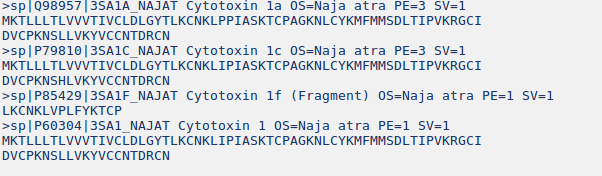
\includegraphics[width=0.8\textwidth]{./images/secuencias.png}
    \caption{Secuencias de varias proteínas en formato \textbf{.fasta}}
    \label{fig:image4}
\end{figure}


La cantidad de información de péptidos que actualmente está guardada es mucha y muy diversa, llegando a un total de 90 millones de proteínas para la base de datos de UniProt. Descargar esta información al completo y procesarla tomaría una gran cantidad de tiempo ya que el archivo superaría los 40 GB de tamaño, esto implicaría un problema importante para realizar diversas tareas de búsqueda. Una de estas tareas consiste es buscar secuencias de aminoácidos (residuos de aminoácidos o \textit{aminoacid residues (AAR)} en inglés) en el conjunto universo de las polipéptidos para poder localizar cuáles son los residuos de ciertos tamaños que más aparecen en las bases de datos. El problema principal radica en buscar cuántas veces aparece cierto residuo de una base de datos que posean tamaños bastante considerables (por ejemplo, buscar una determinada subsecuencia de 2 aminoácidos en una base de datos de 500 GB o superior) sin saber si este residuo está presente o no en aquella proteína, esto podría provocar gastos innecesarios de tiempo a la hora de realizar este tipo de búsqueda, por consiguiente se desea ocupar el menor tiempo posible para realizar esta tarea.

\section{Objetivos}

Lo que se pretende realizar para esta memoria consiste en obtener de un conjunto predeterminado de proteínas lo siguiente:

\begin{enumerate}

\item el número máximo de fragmentos de péptidos (AAR) que existen asociado a un valor $k$ determinado, donde $k$ se ubicará en el intervalo entre 1 hasta 50.
\item En base a lo anterior, obtener y determinar para cada $k$ cuáles son los fragmentos de aminóácidos que más se repiten.

\end{enumerate}

Una vez obtenidos estos datos se realizará un análisis algoritmico y biológico (de manera muy superficial) de los resultados logrados. Para realizar esta tarea se usarán 4 \textit{datasets}:
 
\begin{enumerate}

\item La base de datos de proteínas UniProt-SwissProt \cite{swissprot} (555426 proteínas)
\item La base de datos de proteínas UniProt-TrEMBL \cite{trembl} (88032926 proteínas).
\item La base de datos de péptidos EROP-Moscow \cite{eropmoscow} (14875 oligopéptidos).
\item Las proteínas humanas ingresadas manualmente a la base de datos UniProt (datos extraídos de UniProt-SwissProt, 86298 proteínas). Para este caso solo se considerará $k=1$.

\end{enumerate}

%archivo estado del arte
\chapter{Estado del Arte}

\section{Información previa a considerar}

Para entrar de lleno en la tema, es necesario conocer de antemano varios aspectos básicos de la biología.

\subsection{Biomoléculas}

Cada vez que se habla de la biología, este concepto se relaciona directamente con la ciencia que estudia a los seres vivos. Ahora bien, las estructuras o compuestos que constituyen una parte esencial de los seres vivos son conocidas como \textbf{biomoléculas}. Estas biomoléculas están principalmente constituidas por elementos químicos como el carbono (C), hidrógeno (H), oxígeno (O), nitrógeno (N), fósforo (P) y azufre (S) \cite{biomolecula} y se pueden clasificar en biomoléculas inorgánicas, que se encuentran tanto en seres vivos como en los cuerpos inertes, no obstante son imprescindibles para la vida; y las biomoléculas orgánicas, que son sintetizadas por los seres vivos y tienen una estructura con base en carbono. Estas biomoléculas orgánicas se pueden separar en 4 grandes grupos:
\begin{enumerate}
\item Glúcidos (hidratos de carbono o carbohidratos): son la fuente de energía primaria que utilizan los seres vivos para realizar sus funciones vitales. Los ejemplos más conocidos son la glucosa, el almidón y el glucógeno.
\item Lípidos: conforman el principal almacén de energía de los animales y desempeñan funciones reguladores de enzimas y hormonas.
\item Ácidos nucleicos: El ácido desoxirribonucleico y el ácido ribonucleico, mayormente conocidos como ADN (DNA) y ARN (RNA y sus derivados) desarrollan posiblemente la función más importante para la vida: contener, de manera codificada, las instrucciones necesarias para el desarrollo y funcionamiento de la célula. El ADN tiene la capacidad de replicarse, transmitiendo así dichas instrucciones a las células hijas que heredarán la información.
\item Proteínas: poseen la mayor diversidad de funciones que realizan en los seres vivos; prácticamente todos los procesos biológicos dependen de su presencia y/o actividad. Son proteínas casi todas las enzimas, catalizadores de reacciones metabólicas, hemoglobina, anticuerpos, entre otros. Su unidad base es el {\it{aminoácido}}, por el cual se van formando los péptidos según la cantidad de unidades bases enlazadas.
\end{enumerate}

Dentro de estas biomoléculas, el análisis detallado de los carbohidratos y los lípidos depende en demasía de su estructura química (elementos químicos asociados y tipo de enlaces entre ellos), por lo mismo es una materia más ligada a los químicos (ver Figura 1.1). 

\begin{figure}[H] 

\begin{subfigure}{0.5\textwidth}
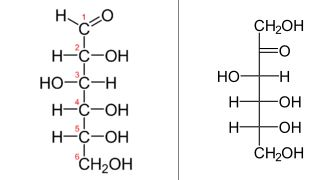
\includegraphics[width=0.9\linewidth, height=5cm]{./images/glucidoejemplos} 
\caption{Glúcidos (glucosa y fructosa)}
\label{fig:subim1}
\end{subfigure}
\begin{subfigure}{0.4\textwidth}
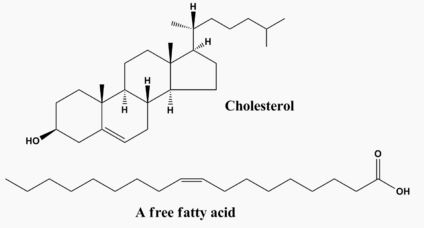
\includegraphics[width=1\linewidth, height=5cm]{./images/lipidosejemplos}
\caption{Lípidos (colesterol y un ácido graso)}
\label{fig:subim2}
\end{subfigure}
 
\caption{Estructura química de los carbohidratos y lípidos.}
\label{fig:image1}
\end{figure}

Sin embargo, el ADN y los polipéptidos poseen unidades base que pueden ser codificadas como letras, por consiguiente pueden ser secuenciados como {\it{cadenas de strings}} y en donde los avances computacionales y la evolución informática toman una importante relevancia (ver Figura 1.2).

\begin{figure}[H]

\begin{subfigure}{0.5\textwidth}
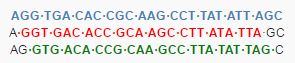
\includegraphics[width=1\linewidth, height=2cm]{./images/adnejemplo}
\caption{Cadena de ADN aleatoria}
\label{fig:subim4}
\end{subfigure}
\begin{subfigure}{0.4\textwidth}
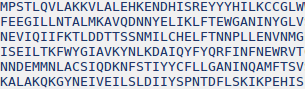
\includegraphics[width=1\linewidth, height=3cm]{./images/cadenaproteina} 
\caption{Cadena aleatoria de una proteína}
\label{fig:subim3}
\end{subfigure}
 
\caption{Biomoléculas de ADN y péptidos llevadas a cadenas de strings.}
\label{fig:image2}
\end{figure}

Con respecto a estas 2 últimas estructuras, la diferencia visual más notoria radica en la cantidad de diferentes letras (strings) que las componen, para el ADN son 4 [8] y son denominadas \textbf{bases nitrogenadas} que son las siguientes:

\begin{enumerate}
\item Adenina
\item Timina
\item Citosina
\item Guanina
\end{enumerate}

Para las proteínas, su elemento básico, como ya se mencionó anteriormente es el \textbf{aminoácido}, pero ahora se adentrará en más detalle sobre esta molécula.

\subsection{Aminoácidos}

Los aminoácidos tienen diferentes funciones en el organismo \cite{amino} pero ante todo sirven como \textbf{las unidades básicas de los péptidos y de las proteínas.} A nivel orgánico el aminoácido es una molécula compuesta con un grupo amino (-NH2) y un grupo carboxilo (-COOH) y que pueden tener distintas distribuciones. Para el caso de los que componen las proteínas se consideran como alfa-aminoácidos:

\begin{figure}[h]
    \centering
    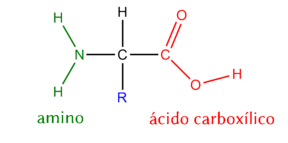
\includegraphics[width=0.4\textwidth]{./images/aminoacido}
    \caption{Estructura general de un alfa-aminoácido}
    \label{fig:image3}
\end{figure}

En la imagen anterior se puede identificar el carbono central (alfa) unido al grupo carboxilo (rojo), grupo amino (verde), un hidrógeno (imagen superior color negro) y el grupo radical (azul) o R. Este grupo radical es el que determina la identidad y las propiedades de cada uno de los diferentes aminoácidos.

El primer aminoácido fue descubierto a principios del siglo XIX, y a partir de ese entonces hasta la actualidad son miles los aminoácidos que han sido descubiertos, pero solo 20 se consideran como los componentes esenciales para las proteínas (y los que se considerarán como parte de esta memoria) que se presentarán a continuación en conjunto con su respectiva abreviación utilizada en las cadenas de proteínas de los archivos FASTA \cite{fasta}:

\begin{table}[H]
\centering
\label{my-label5}
\begin{tabular}{|l l l l|}
\hline
\multicolumn{4}{|c|}{Aminoácido - Abreviatura}\\ \hline
Alanina - A      & Cisteína - C       &      Ácido aspártico - D     & Ácido glutámico - E                     \\
Fenilalalina - F      &  Glicina - G           & Histidina - H     & Isoleucina - I                \\
Lisina - K      & Leucina - L            & Metionina - M           & Aspargarina - N          \\
Prolina - P      & Glutamina - Q          & Arginina - R                  & Serina - S                  \\
Treonina - T      & Valina - V          & Triptófano - W                      & Tirosina - Y   \\ \hline
\end{tabular}
\caption{Los 20 aminoácidos existentes y considerados}
\end{table}

Existen otras abreviaturas en las cadenas como B, X o J, pero para el alcance de esta memoria no serán considerados como objeto de estudio y análisis posterior.

A partir de este pequeño elemento se forman las macromoléculas que se identifican según la cantidad de aminoácidos (a partir de ahora se mencionarán como aa.) que lo compongan:

\begin{table}[H]
\centering
\label{my-label1}
\begin{tabular}{|c|c|}
\hline
Tamaño & \multicolumn{1}{c|}{Tipo de estructura}  \\ \hline
2 aa.     & Dipéptido        \\
3 aa.     & Tripéptido                         \\
Entre 2 y 8 aa.      &      Oligopéptido                             \\
Menos de 100 aa.      &   Péptido       \\
Mayor o igual de 100 aa.   &   Proteína o polipéptido            \\ \hline
\end{tabular}
\caption{Identificación de macromoléculas según cantidad de aminoácidos}
\end{table}

\section{Secuencias de proteínas}

Desde el momento en que se descubrieron los elementos componentes del ADN y las proteínas, se han investigado sobre las posibles combinaciones que se pueden encontrar entre las bases que los conforman y en que cantidad se encuentran. Para el ADN y sus 4 elementos básicos existen millones de seres vivos, parásitos, virus, protozoos y entre otros que se definen por su código genético, por lo cual encontrar los diversos residuos de bases según un determinado tamaño. En el caso puntual para la finalidad de este escrito y según lo mencionado por \cite{zamyatnin1}, es posible estudiar de manera teórica y con fórmulas matemáticas la cantidad máxima de fragmentos que puede formar una proteína. Considerando como base que el número posible de estructuras peptídicas naturales $P$ están compuestas de diferentes residuos de aminoácidos (incluyendo repeticiones en cadenas de aminoácidos) sigue la siguiente fórmula:

\begin{equation}
P=A^{n}
\end{equation}

Donde $A$ es el número de diferentes aminoácidos existentes, y $n$ es la cantidad de aminácidos correspondientes a la estructura estudiada. Por lo mismo y siguiendo esta fórmula (considerando $A=20$) la cantidad de diferentes combinaciones péptidos de tamaño k que se pueden obtener se aprecian en la siguiente Tabla:

\begin{table}[H]
\centering
\label{my-label2}
\begin{tabular}{|c|c|}
\hline
Tamaño péptido (k) & \multicolumn{1}{c|}{Combinaciones posibles ($A^{k}$)}  \\ \hline
2 aa.     & 400        \\
3 aa.     & 8000                         \\
4 aa.      &      160000                             \\
5 aa.      &   3200000       \\
10 aa.      &   1.024$\times 10^{13}$       \\
20 aa.      &   1.049$\times 10^{26}$       \\
50 aa.   &     1.126$\times 10^{65}$   \\ \hline
\end{tabular}
\caption{Combinaciones posibles a obtener según el tamaño del péptido}
\end{table}

Según lo observado en esta Tabla se identificar que a medida que el valor de k va en aumento, las posibles combinaciones que se pueden obtener de fragmentos de proteínas pueden llegar a tener valores inimaginables para el ser humano corriente; no obstante, no todas estas estructuras existen o son capaces de ser encontradas en la naturaleza \cite{array}, aun así la diversidad de la búsqueda de estos residuos sigue siendo gigantesca, y por ende difícil de solucionar, y este será uno de los problemas que se intentará solucionar en esta memoria.

Ahora bien, para un polipéptido de tamaño $n$ aminoácidos, el máximo número posible de fragmentos de tamaño $k$, que teóricamente se podrían obtener (considerando las posibles repeticiones de fragmentos), es descrita mediante la siguiente expresión:

\begin{equation}
N_{k}^{teorica}=n-k+1
\end{equation}

Por consecuencia, el máximo número posible de fragmentos (con repeticiones) que teóricamente se pueden obtener para una molécula de tamaño $n$, partiendo desde $k=2$ (dipéptidos) hasta $k=n-1$, viene dado por:

\begin{equation}
N_{max}^{teorica}=\sum_{2}^{n-1} \frac{k(k-1)}{2}-1
\end{equation}

Mediante estas fórmulas, se han calculado la cantidad de posibles fragmentos que se pueden obtener en diferentes oligopéptidos y proteínas:

\begin{table}[H]
\centering
\label{my-label3}
\begin{tabular}{|c|l|r|r|}
\hline
Número & \multicolumn{1}{c|}{Oligopéptido/Proteína} & \multicolumn{1}{c|}{$n$} & \multicolumn{1}{c|}{$N_{suma}^{teorica}$} \\ \hline
1      & Encefalina (varios tipos biológicos)       & 5                        & 9                     \\
2      & Bradiquinina (mamíferos)                   & 9                        & 35                    \\
3      & ACTH (humanos)                             & 39                       & 740                   \\
4      & Cadena $\alpha$ hemoglobina (humanos)          & 141                      & 9869                  \\
5      & Cadena $\beta$ hemoglobina (humanos)          & 146                      & 10584                 \\ \hline
\end{tabular}
\caption{Número máximo posible de fragmentos que se pueden formar en 5 proteínas}
\end{table}

Considerando que para un polipéptido de largo $n$ aminoácidos, si este valor de $n$ es muy alto, se puede obtener una cantidad muy alta de fragmentos de dipéptidos, pero muchos de estos dipéptidos se pueden repetir varias veces en la cadena, por lo tanto, cuando se desea obtener {\bf{el máximo número de fragmentos diferentes}} asociado a un valor $k$ determinado, este puede tener un valor muy bajo en comparación con la cantidad total de fragmentos obtenidos. Por medio de las fórmulas descritas anteriormente, se puede obtener el número máximo de diferentes fragmentos (o fragmentos esperables) asociado a un tamaño $k$:

\begin{equation}
N_{k}^{diff}=N_{k}^{teorica}- R_{k}
\end{equation}

Este valor $R_{k}$, se obtiene introduciendo nuevos parámetros $i$ (que es el número de estructuras idénticas para determinado $k$) y $m$ (el número de diferentes estructuras para el determinado $k$):

\begin{equation}
R_{k}=\sum_{1}^{m}(i-1)
\end{equation}

Por lo tanto, el número máximo de fragmentos diferentes que se pueden obtener en una proteína sigue la siguiente fórmula:

\begin{equation}
N_{max}^{diff}=\Bigg[\sum_{2}^{n-1} \frac{k(k-1)}{2}-1\Bigg]- \sum_{2}^{n-1}\Bigg[\sum_{1}^{m}(i-1)\Bigg]
\end{equation}
\\
Tomando la información de la base de datos de oligopéptidos EROP-Moscow, para mostrar los valores obtenidos con estas fórmulas, se usará como ejemplo la caseína bovina (proteína proveniente de la vaca). Esta proteína se compone de 4 subunidades, $\alpha - s1$, $\alpha -s2$, $\beta$ y $\kappa$. La siguiente Tabla muestra las cantidades teóricas y diferentes de fragmentos obtenidos como dipéptidos y sus sumas totales:

\begin{table}[H]
\centering
\label{my-label4}
\begin{tabular}{|c|l|c|c|c|c|c|}
\hline
Número & \multicolumn{1}{c|}{Caseína bovina (subunidad)} & $n$ & $N_{2}^{teorica}$ & \multicolumn{1}{l|}{$N_{2}^{diff}$} & \multicolumn{1}{l|}{$N_{max}^{teorica}$} & \multicolumn{1}{l|}{$N_{max}^{diff}$} \\ \hline
1      & $\alpha - s1$                                   & 199 & 198               & 134                                 & 19700                                     & 19621                                  \\
2      & $\alpha - s2$                                   & 207 & 206               & 131                                 & 21320                                     & 21216                                  \\
3      & $\beta$                                         & 209 & 208               & 124                                 & 21735                                     & 21641                                  \\
4      & $\kappa$                                        & 169 & 168               & 118                                 & 14195                                     & 14138                                  \\
5      & $\alpha - s1 + \alpha - s2 + \beta + \kappa$    & 784 & 780               & 260                                 & 76950                                     & 76304                                  \\ \hline
\end{tabular}
\caption{Número máximo posible de fragmentos que se pueden obtener en una proteína de caseína bovina.}
\end{table}

Se puede identificar que para los fragmentos de dipéptidos, la cantidad de diferentes fragmentos es bastante menor que la cantidad total de fragmentos obtenidos para las 4 subunidades, pero aún así la cantidad de fragmentos diferentes totales obtenidos es prácticamente la misma que la cantidad de fragmentos totales sin diferenciar. Esto es notorio ya que si $k$ va en progresivo aumento, el universo combinatorio de posibles fragmentos formados se acorta drásticamente, lo que también favorece a la baja formación de fragmentos que se repiten.

\section{Base de datos UniProt}

UniProt (nombre que proviene de \textit{\textbf{Uni}versal \textbf{Prot}ein}) es una base de datos de secuencias de proteínas e información funcional respectiva, accesible de manera gratuita a todo público. Su fuente de investigación la compone un consorcio cuyos participantes son el Instituto Europeo de Bioinformática (EBI - \textit{European Bioinformatics Institute}), el Instituto Suizo de Bioinformática (SIB - \textit{Swiss Institute of Bioinformatics}) y los Recursos de Información de Proteínas (PIR - \textit{Protein Information Resource}) quienes compusieron UniProt en Diciembre del 2003. Cada uno de estos consorcios está altamente envuelto en las anotaciones y mantenimiento de las bases de datos que corresponden a UniProt, gracias a eso nace \textbf{UniProtKB} (UniProt Knowledgebase), que es una base de datos de proteínas comisariada por expertos, que se compone de 2 secciones:


\begin{enumerate}

\item \textbf{UniProt - SwissProt}: es una base de datos de secuencias de proteínas manualmente anotadas y revisadas. Combina información extraída de la literatura científica y un posterior análisis computacional. Actualmente está compuesto de 555.594 secuencias de proteínas que equivalen a un texto con un peso de 298 MB.

\item \textbf{UniProt - TrEMBL}: es una base de datos de secuencias de proteínas automáticamente anotadas y no revisadas. Estas secuencias son registros de alta calidad y computacionalmente analizados. Esta base de datos fue introducida en respuesta para aumentar el flujo de datos que se obtienen de los proyectos relacionados al genoma. Actualmente está compuesto 90.050.711 secuencias de proteínas que equivalen a un texto con un peso de 40 GB.

\end{enumerate}

\begin{figure}[!htb]
    \centering
    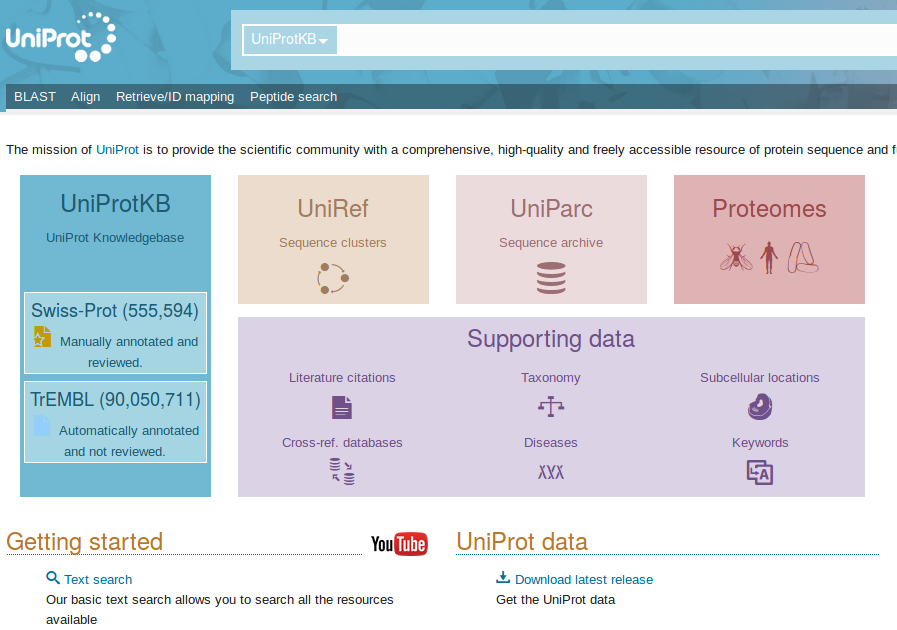
\includegraphics[width=0.8\textwidth]{./images/uniprot_main.png}
    \caption{Página principal del sitio web de UniProt}
    \label{fig:image7}
\end{figure}

\section{Base de datos EROP-Moscow}

EROP-Moscow es una base de datos de secuencias de oligopéptidos de tamaño que rondan entre 2 a 50 aminoácidos altamente detalladas. Fue creada por Alexander Zamyatnin el año 2003 y de manera constante se le agregan nuevas secuencias investigadas \cite{eropmoscow}.

\begin{figure}[h]
    \centering
    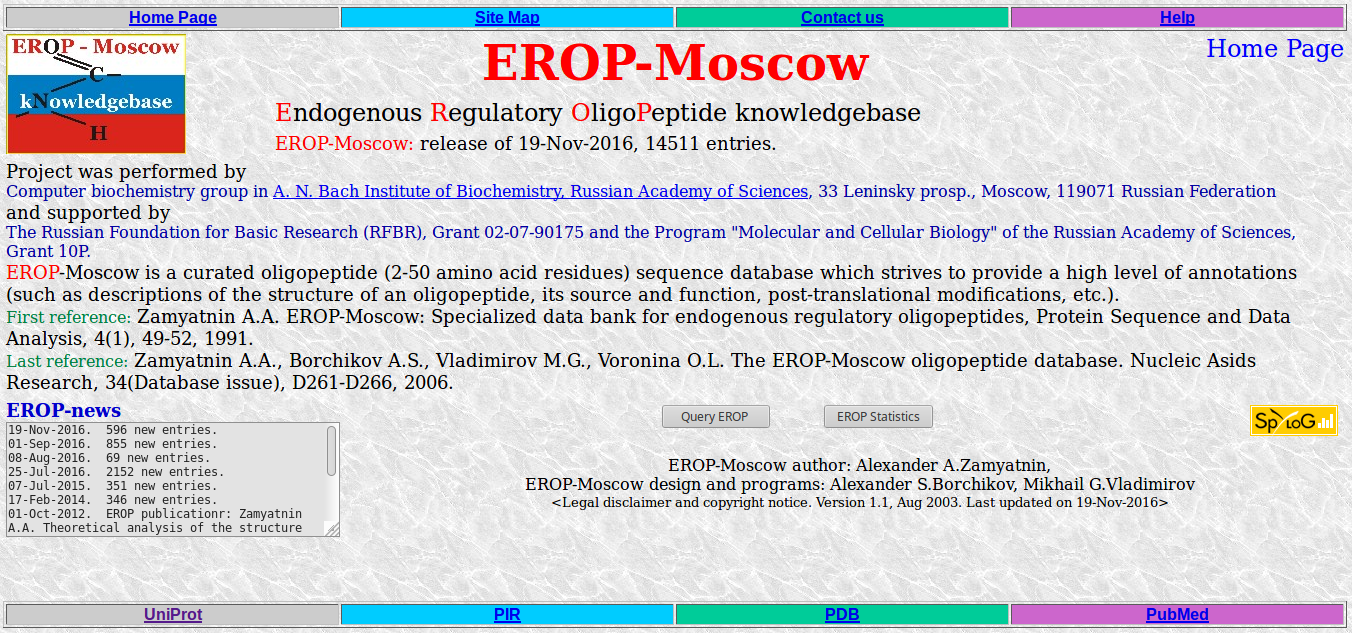
\includegraphics[width=0.8\textwidth]{./images/eropmoscow_main.png}
    \caption{Página principal del sitio web de EROP-Moscow.}
    \label{fig:image8}
\end{figure}

Actualmente está compuesta por 14.785 secuencias que equivalen a un texto con peso de 1.4 MB. Aunque son bastante pocas secuencias en comparación con UniProt, estos péptidos están descritos de manera muy completa y son ideales para realizar diferentes tipos de análisis, ya sea por sus propiedades regulatorias en los seres vivos, propiedades físico-químicas y el tipo de órgano en el cual se encuentran, entre otros.

\section{Técnicas utilizadas en el problema}

En \cite{searching} se menciona que buscar secuencias de proteínas en un predeterminado archivo (puede ser de texto o .fasta) es una tarea muy compleja, ya que se formaría un escenario similar al buscar una {\textit{aguja en un pajar}} y recorrer millones de secuencias en cada búsqueda no sería lo más convieniente considerando que la cantidad de proteínas que existen el día de hoy son muchas, por consiguiente una herramienta recomendable sería preprocesar la base de datos de proteínas con alguna técnica conocida o implementada. A continuación se hablará de forma general de algunos algoritmos conocidos que han tratado este problema.

\subsection{Algoritmo de fuerza bruta}

Este es el algoritmo más simple posible \cite{fuerzabruta}, ya que dado un texto de tamaño \textit{n} se revisan todas las posiciones posibles de un patrón de tamaño \textit{k $<$ n} desde el comienzo hasta el final del texto (izquierda a derecha). Para el caso puntual de los archivos .fasta de las proteínas es necesario extraer únicamente las cadenas de secuencias respectivas y adjuntarlas línea a línea (de esa forma es más fácil trabajarlas). Luego, y siguiendo la presunción matemática del número máximo de fragmentos de tamaño \textit{k} cada una de las cadenas se revisa desde la posición 0 hasta la posición \textit{n-1} (el valor de \textit{n} varía según el largo de la cadena de cada proteína) yendo de caracter a caracter un total de \textit{n-k+1} veces para cada secuencia. Lo siguiente muestra una implementación simple en lenguaje C++ acomodada para obtener los diferentes substrings de largo \textit{k} en un texto de proteínas:
\\
\begin{lstlisting}[language=C++, caption=Búsqueda utilizando fuerza bruta en C++]
set <string> unicos;
ifstream proteinas("proteinas.txt"); //nombre generico
string secuencia;
for (int j = 0; j < cantidad_ss; j++)
{
    getline(proteinas, secuencia);
    int n = secuencia.size();
    int maximo = n-k+1; // k entre 1 a 50
    for (int i = 0; i < maximo; i++)
    {
        string pruebas = secuencia.substr(i,k);
        if (pruebas.find_first_of("BOUXZ")==std::string::npos)
        {
            unicos.insert(pruebas);
        }
    }
}
cout << unicos.size() << endl;
\end{lstlisting}

Haciendo un resumen de este código lo que hace es agregar TODOS los substrings totales de tamaño \textit{k} que encuentra en un string moviéndose letra por letra y se verifica si el substring no posee algún aminoácido que no se encuentre dentro de los 20 aa. mencionados anteriormente, en caso afirmativo el substring se ingresa al set (estructura cuya cualidad es no repetir elementos en su conjunto). Una vez realizado todo esto se puede obtener el número de diferentes substrings de tamaño $k$ que se encuentran en el texto, que es la gran ventaja que posee esta implementación, por lo que puede servir como un ``verificador de resultados'' cuando se analicen los resultados de implementaciones más óptimas.

Como desventajas importantes resalta el hecho de que el tiempo de la implementación es muy lento ya que al saltar letra por letra y realizando todas las comparaciones posibles de los substrings se pierde bastante tiempo (la complejidad es de $O(n-k+1)$ por cadena, si se tiene que $N$ es la cantidad total de proteínas la complejidad en el texto sería de $O(N(n-k+1))$), que también es negativamente afectado por el tamaño del texto a trabajar (usar un texto de 40 GB como el ``uniprot\_trembl.fasta'' demoraría casi 20 horas en obtener los diferentes substrings para un \textit{k = 15}). Además para guardar un \texttt{set$<$string$>$} en C++ requiere de una gran capacidad de memoria RAM, la cual va peligrosamente en aumento si \textit{k} sube su valor. Por otra parte esta implementación tampoco entrega la factibilidad de encontrar una manera de extraer aquellos substrings de tamaño $k$ que más se repiten. Por consiguiente esta implementación básica no ayuda a realizar por completo la tarea esperada para este trabajo. 


\subsection{Algoritmos de búsqueda de strings}

Esta clase de algoritmos (en inglés conocidos como \textit{string searching algorithm}) tratan de localizar si uno o varios strings solicitados (que también se llaman patrones) aparecen en un string más largo o simplemente un texto como tal, considerando el alfabeto que por el cual está compuesto el string de destino o texto. En la mayoría de las ocasiones este alfabeto ($\Sigma$) es el que determina el rendimiento de determinado algoritmo (una variación de este alfabeto puede ayudar o perjudicar la eficiencia de un algoritmo en particular), como también el texto a analizar.
Una clasificación básica de estos algoritmos se puede realizar según la cantidad de strings a encontrar:
\begin{enumerate}
\item Algoritmos de búsqueda de un único patrón (\textit{Single pattern algorithms})
\item Algoritmos de búsqueda de múltiples patrones (\textit{Multiple pattern algorithms})
\end{enumerate}

\subsubsection{Algoritmos de búsqueda de un único patrón}
Como lo dice el mismo título y hablando de manera más formal, esta clase de algoritmo de búsqueda consiste en encontrar las ocurrencias de un determinado patrón \cite{stringmatching} $p=p_{1}p_{2}$ $\ldots$ $p_{m}$ en un texto largo $T=T_{1}T_{2}$ $\ldots$ $T_{n}$, donde $p$ y $T$ son secuencias de caracteres que provienen de set finito de caracteres $\Sigma$.
Para este caso se describirán de manera sencilla los algoritmos más reconocidos que han sido desarrollados para este problema, que son el algoritmo de \textbf{Knuth-Morris-Pratt} y el algoritmo de \textbf{Boyer-Moore}.

$a)$ \textbf{Algoritmo de Knuth-Morris-Pratt}

Este algoritmo desarrollado el año 1977 por Donald E. Knuth, James H. Morris, y Vaughan R. Pratt busca como objetivo minimizar la cantidad de comparaciones del patrón \textit{p} con el texto \textit{T} manteniendo una pista de información obtenida en informaciones previas, valiéndose de la ayuda de una función de fallo (preproceso del patrón) que indica cuando la última comparación se puede reusar si existe un fallo (revisar \cite{knuthmorrispratt} para mayores detalles). Las comparaciones de caracteres se realizan de izquierda a derecha buscando el prefijo más largo posible y usarlo como información importante en las iteraciones siguientes (pseudocódigo en sección Apéndice, algoritmo \ref{alg:algoritmo1}). Se puede tomar como ejemplo el texto ``aaaabaabaaab'' y el patrón ``aabaaa''.
\\
\begin{table}[h]
\centering
\label{my-label6}
\begin{tabular}{lllllllllllll}
\cline{2-13}
\multicolumn{1}{l|}{T:} & \multicolumn{1}{l|}{a} & \multicolumn{1}{l|}{a} & \multicolumn{1}{l|}{a}                         & \multicolumn{1}{l|}{a}                         & \multicolumn{1}{l|}{b} & \multicolumn{1}{l|}{a}                         & \multicolumn{1}{l|}{a}                         & \multicolumn{1}{l|}{b}                         & \multicolumn{1}{l|}{a}                         & \multicolumn{1}{l|}{a}                         & \multicolumn{1}{l|}{a}                         & \multicolumn{1}{l|}{b} \\ \cline{2-13} 
\multicolumn{1}{l}{P1:}   & \multicolumn{1}{l}{a} & \multicolumn{1}{l}{a} & \multicolumn{1}{l}{\cellcolor[HTML]{FD6864}b} &                                                &                        &                                                &                                                &                                                &                                                &                                                &                                                &                        \\ 
P2:               & \multicolumn{1}{l}{}  & \multicolumn{1}{l}{a} & \multicolumn{1}{l}{a}                         & \multicolumn{1}{l}{\cellcolor[HTML]{FD6864}b} &                        &                                                &                                                &                                                &                                                &                                                &                                                &                        \\
  P3:                      &                        & \multicolumn{1}{l}{}  & \multicolumn{1}{l}{a}                         & \multicolumn{1}{l}{a}                         & \multicolumn{1}{l}{b} & \multicolumn{1}{l}{a}                         & \multicolumn{1}{l}{a}                         & \multicolumn{1}{l}{\cellcolor[HTML]{FD6864}a} &                                                &                                                &                                                &                        \\
 P4:                    &                        &                        &                                                &                                                & \multicolumn{1}{l}{}  & \multicolumn{1}{l}{\cellcolor[HTML]{9AFF99}a} & \multicolumn{1}{l}{\cellcolor[HTML]{9AFF99}a} & \multicolumn{1}{l}{\cellcolor[HTML]{9AFF99}b} & \multicolumn{1}{l}{\cellcolor[HTML]{9AFF99}a} & \multicolumn{1}{l}{\cellcolor[HTML]{9AFF99}a} & \multicolumn{1}{l}{\cellcolor[HTML]{9AFF99}b} &                        \\        
\end{tabular}
\caption{Ejemplo de uso del algoritmo de Knuth-Morris-Pratt}
\end{table}

Apreciando la imagen se puede identificar que el algoritmo KMP realiza un total de 14 comparaciones hasta encontrar que el patrón aparece en el texto, en el caso de la fuerza bruta hubiesen sido necesarias 21 comparaciones hasta identificar que el patrón está en el texto.
El tiempo de preprocesamiento del texto va del orden $O(m)$ donde $m$ es el largo del patrón, y el tiempo que demora el patrón en ser ubicado en el texto es aproximadamente del orden $O(n)$ donde $n$ es el largo del texto.

$b)$ \textbf{Algoritmo de Boyer-Moore}

Este algoritmo desarrollado por Bob Boyer y J. Strother Moore el año 1977 se desmarca del algoritmo KMP ya que para Boyer-Moore se realiza la comparación entre patrón y texto de derecha a izquierda, por ejemplo si hubiera una discrepancia en el último carácter del patrón y el carácter del texto no aparece en todo el patrón, entonces éste se puede deslizar $m$ posiciones sin realizar ninguna comparación extra. En particular, no es necesario comparar los primeros $m-1$ caracteres del texto, lo cual indica que podría realizarse una búsqueda en el texto con menos de $n$ comparaciones; sin embargo, si el carácter discrepante del texto se encuentra dentro del patrón, éste podría desplazarse en un número menor de espacios \cite{boyermoore}. Esto le entrega una gran ventaja de tiempo y espacio en comparación al algoritmo KMP, en especial cuando el patrón analizado es grande (compuesto por más de 10 caracteres). Para ello se vale de la ayuda de un preprocesamiento del patrón para obtener la posición de ocurrencia de cada uno de los diferentes caracteres involucrados y un localizador de sufijos (pseudocódigo en sección Apéndice, algoritmo \ref{alg:algoritmo2}). Ahora bien, volviendo a realizar la comparación tomando el texto ``aaaabaabaaab'' y el patrón ``aabaaa'': 

\begin{table}[h]
\centering
\label{my-label7}
\begin{tabular}{lllllllllllll}
\cline{2-13}
\multicolumn{1}{l|}{T:}  & \multicolumn{1}{l|}{a}                         & \multicolumn{1}{l|}{a}                         & \multicolumn{1}{l|}{a}                         & \multicolumn{1}{l|}{a}                         & \multicolumn{1}{l|}{b}                         & \multicolumn{1}{l|}{a}                         & \multicolumn{1}{l|}{a}                         & \multicolumn{1}{l|}{b}                         & \multicolumn{1}{l|}{a}                         & \multicolumn{1}{l|}{a}                         & \multicolumn{1}{l|}{a}                         & \multicolumn{1}{l|}{b} \\ \cline{2-13} 
\multicolumn{1}{l}{P1:} & \multicolumn{1}{l}{a} & \multicolumn{1}{l}{a} & \multicolumn{1}{l}{b} & \multicolumn{1}{l}{a} & \multicolumn{1}{l}{\cellcolor[HTML]{FD6864}a} & \multicolumn{1}{l}{\cellcolor[HTML]{9AFF99}a} &                    &       &                       &        &                       &                        \\
P2:                      &                       &  & \multicolumn{1}{l}{a} & \multicolumn{1}{l}{a} & \multicolumn{1}{l}{b} & \multicolumn{1}{l}{a} & \multicolumn{1}{l}{a} & \multicolumn{1}{l}{\cellcolor[HTML]{FD6864}a} &              &               &                     &                        \\
P3:                      &                       &                       &                        &                      &  & \multicolumn{1}{l}{\cellcolor[HTML]{9AFF99}a} & \multicolumn{1}{l}{\cellcolor[HTML]{9AFF99}a} & \multicolumn{1}{l}{\cellcolor[HTML]{9AFF99}b} & \multicolumn{1}{l}{\cellcolor[HTML]{9AFF99}a} & \multicolumn{1}{l}{\cellcolor[HTML]{9AFF99}a} & \multicolumn{1}{l}{\cellcolor[HTML]{9AFF99}a} &                        \\
\end{tabular}
\caption{Ejemplo de uso del algoritmo de Boyer-Moore}
\end{table}

Para este ejemplo se puede apreciar que con Boyer-Moore se realizan 9 comparaciones totales hasta finalmente encontrar que el patrón está ubicado en el texto, mejorando el resultado de Knuth-Morris-Pratt.
Este algoritmo tiene un tiempo de preprocesamiento del orden de $O(m+k)$ donde $m$ es el largo del patrón y $k$ es cantidad de elementos que componen el alfabeto utilizado; el tiempo que demora en encontrar el patrón en el texto varía entre el orden $O(n/m)$ para el mejor caso y el orden $O(nm)$ para el peor caso, considerando $n$ como el largo del texto en cuestión.

Mirando de una visión macro, pareciera ser que estos algoritmos tuvieran un mejor comportamiento a nivel de tiempo y rendimiento que el algoritmo de fuerza bruta, ¿pero son realmente convenientes para aplicarlos a archivos grandes de proteínas en formatos .fasta? Por una parte, estos algoritmos requieren de un \textbf{patrón}, que en este caso serían los posibles residuos de aminoácidos que existen para un tamaño $k$, por consiguiente, hay que ponerse en el caso de que se buscan los diferentes residuos de proteínas de largo 6, que equivalen a comparar las 64.000.000 combinaciones posibles y buscarlas en el archivo, que si es grande (por ejemplo superior a los 100 MB) demoraría mucho tiempo porque en ciertos casos podría ocurrir de que se revise para un solo residuo todo el archivo y no encontrarlo en el texto, en consecuencia revisar a cada rato el archivo desde el principio es un objetivo que se desea evitar para este caso del trabajo.

Casi 40 años han pasado desde que estos 2 algoritmos aparecieron para trabajarlos, sin embargo y con el paso del tiempo han aparecido nuevas mejoras de estas implementaciones (como Horsepool) o simplemente nuevos algoritmos que utilizan acercamientos en base a factores intermedios (como el algoritmo BOM - \textit{Backward Oracle Matching}), aunque estas nuevas implementaciones también caen en lo mismo, volver a utilizar como patrones a todos los potenciales residuos de aminoácidos de largo \textit{k}, y usando valores de \textit{k} muy largos puede ser una tarea infinita de realizar.

\subsubsection{Algoritmos de búsqueda de múltiples patrones}

Esta clase de algoritmos es una extensión del punto anterior, ya que aquí se buscan de manera simultánea si un conjunto de patrones $P=$\{$p_{1}$, $p_{2}$, $\ldots$, $p_{3}$\} aparece en un texto $T$ dado un set de caracteres $\Sigma$ \cite{stringmatching}. Las implementaciones más reconocidas para este caso son el algoritmo de \textbf{Aho-Corsack} (una extensión de algoritmo de Knuth-Morris-Pratt), el algoritmo de \textbf{Commentz-Walter} (una extensión del algoritmo de Boyer-Moore) y el algoritmo de \textbf{Set-BOM} (una extensión del algoritmo \textit{Backward Oracle Matching}). 

Como es lógico, aumentar la cantidad de palabras (patrones) a comparar en el texto determinado toma un proceso más caro a nivel de espacio, pero considerando que se tuviera un gran rango de patrones a buscar, como el caso de todos los potenciales péptidos de tamaño $k$ a encontrar, tomaría una visión mucho más optimista que usando un algoritmo de búsqueda con un solo patrón incluyendo una optimización en los tiempos totales de búsqueda. No obstante, se repetiría el mismo fenómeno con los archivos de gran tamaño, requiriendo de un patrón para localizar y que puede no estar en el texto, lo que supondría un gasto de tiempo innecesario e infructuoso para este trabajo, si esto se traduce en tener muchos substrings para analizarlos como patrones en este caso, por consiguiente utilizar estos algoritmos no es conveniente.



\subsection{Estructuras de datos para texto}

Los casos vistos anteriormente tienen como principal problema que para cada patrón dado, es necesario \textbf{revisar el texto desde el inicio hasta llegar a la ubicación donde el patrón existe o simplemente recorrer el texto completo sin ubicar al patrón}, ejemplificando, sería como tener que llevar 20 ovejas de La Serena a Santiago y se va trasladando de una a una generando una pérdida inmensa de tiempo y costo, por ende tiene mucho más sentido agrupar estas ovejas y luego llevarlas todas juntas a su destino. Por lo tanto lo que se busca en definitiva es \textbf{organizar todos los patrones en una única estructura de datos}, y para lograr esta tarea, no será necesario tener a mano a los patrones a buscar, sino que al \textbf{texto en sí} el cual puede ser agrupado como una larga ``cadena de strings''.

Llevando a un ejemplo más concreto y sencillo, se tiene la palabra MISSISSIPPI\$ que está compuesta por 12 letras o caracteres. Cada caracter se podría representar por medio de un índice (indexar la palabra) y quedaría de la siguiente forma:

\begin{table}[h]
\centering
\begin{tabular}{llllllllllll}
0                       & 1                      & 2                      & 3                      & 4                      & 5                      & 6                      & 7                      & 8                      & 9                      & 10                     & 11                     \\ \hline
\multicolumn{1}{|l|}{M} & \multicolumn{1}{l|}{I} & \multicolumn{1}{l|}{S} & \multicolumn{1}{l|}{S} & \multicolumn{1}{l|}{I} & \multicolumn{1}{l|}{S} & \multicolumn{1}{l|}{S} & \multicolumn{1}{l|}{I} & \multicolumn{1}{l|}{P} & \multicolumn{1}{l|}{P} & \multicolumn{1}{l|}{I} & \multicolumn{1}{l|}{\$} \\ \hline
\end{tabular}
\caption{Índices de la palabra MISSISSIPPI\$}
\end{table}

El concepto \textbf{sufijo} corresponde para este contexto al sector de la palabra desde un punto medio (que puede ser incluso el comienzo de la palabra) hasta el final (el prefijo recurre un sector desde el inicio hasta el punto intermedio), lo cual será útil para el siguiente punto.
A partir de la imagen superior es posible obtener los ``sufijos'' de esta palabra, para posteriormente agrupar todos estos ``sufijos'' e ir ordenándolos alfabéticamente (observar Tabla 2.8 en la siguiente página).

\begin{table}[h]
	\centering
	\label{my-label8}
	\begin{tabular}{c l c c l}
		0 & MISSISSIPPI\$ &  & 11 & \$\\
		1 & ISSISSIPPI\$ &  & 10 & I\$\\
		2 & SSISSIPPI\$ &  & 7 & IPPI\$\\
		3 & SISSIPPI\$ &  & 4 & ISSIPPI\$\\
		4 & ISSIPPI\$ &  & 1 & ISSISSIPPI\$\\
		5 & SSIPPI\$ &  & 0 & MISSISSIPPI\$\\
		6 & SIPPI\$ &  & 9 & PI\$\\
		7 & IPPI\$ &  & 8 & PPI\$\\
		8 & PPI\$ &  & 6 & SIPPI\$\\
		9 & PI\$ &  & 3 & SISSIPPI\$\\
		10 & I\$ &  & 5 & SSIPPI\$\\
		11 & \$ &  & 2 & SSISSIPPI\$\\
	\end{tabular}
\caption{Sufijos (sector izquierdo) e índices (sector derecho) ordenados según orden alfabético.}
\end{table}

La clave de este ordenamiento está en el \textbf{nuevo orden que tienen los índices}, los cuales tendrán una vital importancia a la hora del desarrollo de esta memoria, y que pueden ser implementados a partir de la palabra o texto entregado para luego guardarlos y registrarlos en un vector.

Los algoritmos encargados de trabajar con este tipo de indexación son conocidos como \textbf{Búsqueda de Datos Indexados} (en inglés se conocen como \textit{Indexed Text Searching}) y de los cuales se describirán los más conocidos.

\subsection{Árbol de sufijos}

Para la lectura de las secuencias de proteínas y ADN, actualmente se considera el uso de los árboles de sufijos \cite{pekka} o también conocido como el \textit{suffix tree}, el cual es muy usado para leer cadenas de strings, ya que es ideal para desarrollar diversos problemas relativos al uso de strings como hallar substrings en común, comparación de estadísticas, proyectos relacionados con el genoma, entre otros. \\
Formalmente hablando, el árbol de sufijos \cite{sufijos} es una estructura de datos comprimida que sirve para almacenar una cadena de caracteres con “información pre-procesada” sobre su estructura interna. Según lo definió Weiner en 1973 \cite{pavesi} el árbol de sufijos $\tau$ para un string $S$ de largo $m=s_{1}s_{2}...s_{m}$ posee un nodo de inicio, y nodos hoja o hijos (que serán al menos 2). Comienza leyendo $s_{1}$, luego lee $s_{2}$ (que es $s_{1}$ quitándole la primera letra respectiva desde izquierda a derecha) identificando si hay strings que ya formaron una descendencia similar para continuar por la hoja y no crear otra y en caso contrario crear una nueva hoja, hasta así leer todo el string. En ciertas oportunidades, un sufijo de $S$ podría coincidir con el prefijo de algún otro sufijo de $S$, por lo tanto el camino para el primer sufijo no terminaría en una hoja. Por ello que la solución creada fue añadir un carácter terminador, siendo usado comúnmente el $\$$ para este caso.
\\Esto es muy útil, por ejemplo, para resolver el problema de la subcadena en tiempo lineal ya que se tiene este texto $S$ de longitud $m$ el cual se pre-procesa (se construye el árbol) en tiempo de orden $O(m)$ donde se busca una subcadena $P$ de longitud $n$ (cuyo tiempo es de $O(n)$).

\begin{figure}[h]

\begin{subfigure}{0.5\textwidth}
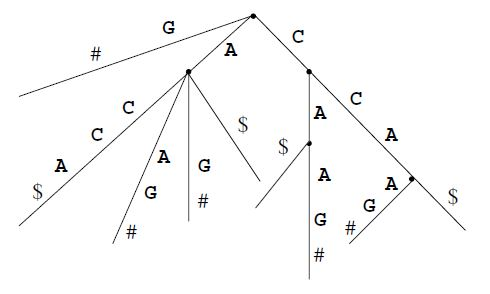
\includegraphics[width=0.9\linewidth, height=5cm]{./images/suffixtree1.JPG} 
\caption{Árbol de sufijos de una cadena de ADN aleatoria}
\label{fig:subim5}
\end{subfigure}
\begin{subfigure}{0.5\textwidth}
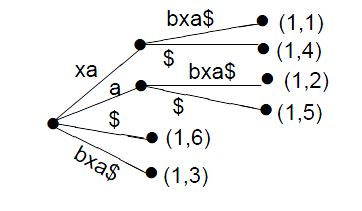
\includegraphics[width=0.9\linewidth, height=5cm]{./images/suffixtree2.JPG}
\caption{Árbol de sufijos de la palabra $xabxa$}
\label{fig:subim6}
\end{subfigure}
 
\caption{Ejemplos de árboles de sufijos.}
\label{fig:image3}
\end{figure}

El problema para la secuencia de ADN considera que habrá un conjunto de textos $S_{i}$ pertenecientes a la cadena de nucleóticos, y en el cual poder verificar si $P$ es subcadena de algún $S_{i}$, lo que es llamado {\it{el árbol de sufijos generalizado}} (ver Figura \ref{fig:mesh1}). 

\begin{figure}[h]
    \centering
    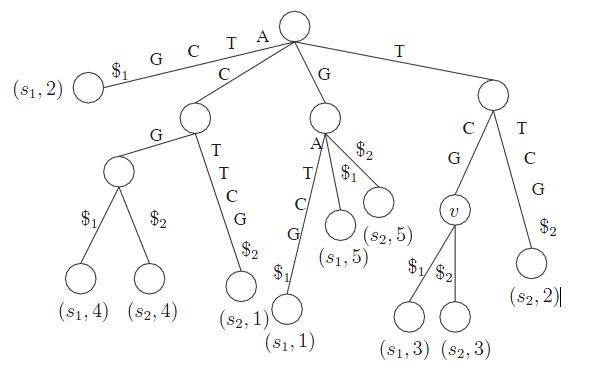
\includegraphics[width=0.55\textwidth]{./images/suffixtree3.JPG}
    \caption{El árbol de sufijo generalizado para las secuencias {\it{GATCG\$}} y {\it{CTTCG\$}} \cite{koaluru}}
    \label{fig:mesh1}
\end{figure}

\subsection{Arreglo de sufijos}

Los arreglos de sufijos fueron introducidos por Udi Mander y Gene Myers el año 1990 \cite{suffixarray1} y corresponden a una variante del árbol de sufijos mucho más eficiente en cuanto al uso de la memoria \cite{licenciado}. 

Hablando de manera más formal, sea $T=t_{1}, t_{2},$ $\ldots$ $,t_{n}$ una cadena y sea $T[i,j]$ la subcadena que va del índice $i$ hasta $j$. El arreglo de sufijos $SA$ de la cadena $T$ va a ser un arreglo de enteros brindando las posiciones iniciales de los sufijos en $T$ en órden lexicográfico. Esto significa que $SA[i]$ contiene la posicion inicial del $i$-ésimo sufijo más pequeño en $T$ y por tanto se cumple que para todo $1 < i \leq n: T[SA[i-1],n] < T[SA[i],n]$. 

Reutilizando el ejemplo de la palabra MISSISSIPPI\$, el arreglo de sufijos que contiene las posiciones iniciales sería el siguiente:

\begin{table}[h]
\centering
\label{my-label9}
\begin{tabular}{|
>{\columncolor[HTML]{EFEFEF}}c|c|c|c|c|c|c|c|c|c|c|c|c|}
\hline
$i$        & 0  & 1  & 2 & 3 & 4 & 5 & 6 & 7 & 8 & 9 & 10 & 11 \\ \hline
$SA{[}i{]}$ & 11 & 10 & 7 & 4 & 1 & 0 & 9 & 8 & 6 & 3 & 5  & 2  \\ \hline
\end{tabular}
\caption{Arreglo de sufijos $A[i]$ de la palabra MISSISSIPPI\$}
\end{table} 

Para este tipo de estructura, y tal como menciona \cite{abeliuk}, encontrar un patrón $P$ de tamaño $m$ (donde $m < n$) en el texto consiste en buscar el intervalo $[j,k]$ en el arreglo que contiene a todos los sufijos que comienzan con el patrón mencionado. Esto se logra mediante una búsqueda binaria sobre $A$, buscando lexicográficamente el menor sufijo que parte con $P$, y otra búsqueda binaria buscando el mayor sufijo que parte con $P$. En cada comparación de esta búsqueda binaria se compara un sufijo con el patrón, lo que toma tiempo $O(m)$ en el peor caso, luego la búsqueda completa toma $O(m \log n)$. Junto con el arreglo de sufijos es necesario guardar el texto, y ambos juntos ocupan $O(n \log n)$ bits de espacio y un tiempo del orden de $O(n (\log n)^{2})$ \cite{suffixarray2} (pseudocódigo en sección Apéndice, algoritmo \ref{alg:algoritmo3}).

\subsubsection*{Diferencias entre árbol de sufijos y arreglo de sufijos}

Ambas estructuras representan (entregan como salida) el mismo resultado, pero con varias discrepancias. La más obvia, es que el \textit{suffix tree} es un árbol donde al recorrer cada una de sus hojas se obtiene el arreglo de sufijos. No obstante, la diferencia importante entre ambos algoritmos radica en \textbf{la cantidad de espacio utilizada}. La construcción del árbol de sufijos toma tiempo lineal en el largo del texto. El árbol de sufijos tiene $O(n)$ nodos. Luego, dado que los substrings de cada rama pueden ser guardados como la posición y el largo de un substring del texto $S$, un árbol de sufijos de $n$ nodos ocupa $O(n \log n)$ bits. Esto permite realizar varias operaciones sobre los nodos del \textit{suffix tree}. Sin embargo esto se convierte en un problema porque implica un tamaño de almacenamiento de varias veces el texto original \cite{abeliuk}. 

Por el contrario el arreglo de sufijos pierde varias de estas funciones a cambio de una importante mejora en cuanto a los requerimientos en espacio de los árboles de sufijos porque el \textit{suffix array} guarda \textbf{$n$ enteros}. Por lo cual si se tiene un arreglo donde un entero requiere 4 $bytes$ (32 bits), un arreglo de sufijos en ese caso requeriría un total de implementación de $4n$ $bytes$ (si el entero necesitara 8 $bytes$ (64 bits), el arreglo tendría un tamaño de $8n$ $bytes$). Y esto es significativamente menor que los $20n$ bytes requeridos en la implementación del árbol de sufijos \cite{kurtz}.

\subsection{Arreglo LCP}

LCP es una sigla en inglés que hace referencia al ``Prefijo común más largo'' (LCP = \textit{Longest Common Prefix}). Este arreglo es una estructura auxiliar al arreglo de sufijos (tamaño igual al del \textit{suffix array}), pero que en sus posiciones guarda las longitudes de los prefijos comunes más largos entre todos los pares de sufijos consecutivos correspondientes al arreglo de sufijos. 

Esta estructura fue introducida el año 1990 por Udi Manber y Gene Myers con la finalidad de optimizar el tiempo de ejecución para la búsqueda de strings \cite{suffixarray1}. Y de manera formal se define como: Se tiene $SA$ que es el arreglo de sufijos del texto $T=t_{0}t_{1}$ $\ldots$ $t_{n-1}$ y $lcp(v,w)$ es el largo del prefijo común más largo entre 2 strings $v$ y $w$. Además se sabe que $T[i,j]$ es el substring de $S$ que va desde la posición $i$ hasta $j$. Por consiguiente el arreglo $LCP[0,n-1]$ es un arreglo compuesto de números enteros de tamaño $n$ donde $LCP[0]$ está indefinido y $LCP[i] = lcp(T[SA[i-1],n], T[SA[i],n])$ para todo $1 < i \leq n$. Por consiguiente $LCP[i]$ almacena la longitud del prefijo común más largo del -lexicográficamente hablando-  $i$-ésimo sufijo más pequeño y su predecesor en el \textit{suffix array}.

Para mostrar un ejemplo, se usará nuevamente la palabra MISSISSIPPI\$ en base al SA obtenido anteriormente, mostrando también sus sufijos ordenados (ver Tabla 2.10). A partir de esto el arreglo LCP es construido comparando lexicográficamente a los sufijos consecutivos para determinar el prefijo común más largo (ver Tabla 2.11).

\begin{table}[!htb]
\centering
\label{my-label10}
\begin{tabular}{|l|l|l|l|l|l|l|l|l|l|l|l|l|}
\hline
\textbf{i}         & \multicolumn{1}{c|}{0}  & \multicolumn{1}{c|}{1}  & \multicolumn{1}{c|}{2} & \multicolumn{1}{c|}{3} & \multicolumn{1}{c|}{4} & \multicolumn{1}{c|}{5} & \multicolumn{1}{c|}{6} & \multicolumn{1}{c|}{7} & \multicolumn{1}{c|}{8} & \multicolumn{1}{c|}{9} & \multicolumn{1}{c|}{10} & \multicolumn{1}{c|}{11} \\ \hline
\textbf{T{[}i{]}}  & \multicolumn{1}{c|}{m}  & \multicolumn{1}{c|}{i}  & \multicolumn{1}{c|}{s} & \multicolumn{1}{c|}{s} & \multicolumn{1}{c|}{i} & \multicolumn{1}{c|}{s} & \multicolumn{1}{c|}{s} & \multicolumn{1}{c|}{i} & \multicolumn{1}{c|}{p} & \multicolumn{1}{c|}{p} & \multicolumn{1}{c|}{i}  & \multicolumn{1}{c|}{\$}  \\ \hline
\textbf{SA{[}i{]}} & \multicolumn{1}{c|}{11} & \multicolumn{1}{c|}{10} & \multicolumn{1}{c|}{7} & \multicolumn{1}{c|}{4} & \multicolumn{1}{c|}{1} & \multicolumn{1}{c|}{0} & \multicolumn{1}{c|}{9} & \multicolumn{1}{c|}{8} & \multicolumn{1}{c|}{6} & \multicolumn{1}{c|}{3} & \multicolumn{1}{c|}{5}  & \multicolumn{1}{c|}{2}  \\ \hline
\textbf{0}                                                       & \$                       & i                       & i                      & i                      & i                      & m                      & p                      & p                      & s                      & s                      & s                       & s                       \\ \hline
\textbf{1}                                                       &                         & \$                       & p                      & s                      & s                      & i                      & i                      & p                      & i                      & i                      & s                       & s                       \\ \hline
\textbf{2}                                                       &                         &                         & p                      & s                      & s                      & s                      & \$                      & i                      & p                      & s                      & i                       & i                       \\ \hline
\textbf{3}                                                       &                         &                         & i                      & i                      & i                      & s                      &                        & \$                      & p                      & s                      & p                       & s                       \\ \hline
\textbf{4}                                                       &                         &                         & \$                      & p                      & s                      & i                      &                        &                        & i                      & i                      & p                       & s                       \\ \hline
\textbf{5}                                                       &                         &                         &                        & p                      & s                      & s                      &                        &                        & \$                      & p                      & i                       & i                       \\ \hline
\textbf{6}                                                       &                         &                         &                        & i                      & i                      & s                      &                        &                        &                        & p                      & \$                       & p                       \\ \hline
\textbf{7}                                                       &                         &                         &                        & \$                      & p                      & i                      &                        &                        &                        & i                      &                         & p                       \\ \hline
\textbf{8}                                                       &                         &                         &                        &                        & p                      & p                      &                        &                        &                        & \$                      &                         & i                       \\ \hline
\textbf{9}                                                       &                         &                         &                        &                        & i                      & p                      &                        &                        &                        &                        &                         & \$                       \\ \hline
\textbf{10}                                                      &                         &                         &                        &                        & \$                      & i                      &                        &                        &                        &                        &                         &                         \\ \hline
\textbf{11}                                                      &                         &                         &                        &                        &                        & \$                      &                        &                        &                        &                        &                         &                         \\ \hline
\end{tabular}
\caption{SA de MISSISSIPPI\$ y sus sufijos respectivos}
\end{table}

Por ejemplo, $LCP[4] = 4$ que es la longitud del prefijo común más largo ISSI que se comparten entre los sufijos $SA[3] = T[4,11] =$ ISSIPPI\$ y $SA[4] = T[1,11] =$ ISSISSIPPI\$. Notar que $LCP[0] = \emptyset$ ya que no hay un sufijo más pequeño lexicográficamente hablando \cite{lcparray}.

\begin{table}[!htb]
\centering
\label{my-label11}
\begin{tabular}{|l|c|c|c|c|c|c|c|c|c|c|c|c|}
\hline
\textbf{i}         & 0  & 1  & 2 & 3 & 4 & 5 & 6 & 7 & 8 & 9 & 10 & 11 \\ \hline
\textbf{T{[}i{]}}  & m  & i  & s & s & i & s & s & i & p & p & i  & \$  \\ \hline
\textbf{SA{[}i{]}} & 11 & 10 & 7 & 4 & 1 & 0 & 9 & 8 & 6 & 3 & 5  & 2  \\ \hline
\textbf{LCP{[}i{]}} & $\emptyset$  & 0  & 1 & 1 & 4 & 0 & 0 & 1 & 0 & 2 & 1  & 3  \\ \hline
\end{tabular}
\caption{Arreglo LCP de la palabra MISSISSIPPI\$}
\end{table}

La construcción del algoritmo del arreglo LCP se puede establecer en 2 categorías, obtener el arreglo LCP como un bi-producto del arreglo de sufijos \cite{suffixarray1} o simplemente utilizar un arreglo de sufijos previamente construído \cite{kasai}. Para este segundo caso el arreglo LCP es construido en un tiempo del orden de $O(n \log n)$, y si se asume que cada simbolo de texto pesa un byte y cada valor o elemento del arreglo de sufijos y arreglo LCP pesa 4 bytes, considerando un texto de tamaño $n$ entonces el peso total para guardar los 2 arreglos sería $8n$ (pseudocódigo en sección Apéndice, algoritmo \ref{alg:algoritmo4}).


\subsection{External Memory Suffix Array}

Como se vio anteriormente, la construcción del \textit{suffix array} (SACA, sigla en inglés de \textit{Suffix Array Construction Algorithm}) se realiza en memoria RAM, donde se almacena el texto de entrada y el posterior arreglo de sufijos. Sin embargo existen textos muy grandes como la base de datos de Wikipedia, bases de datos de genomas, variados textos que superen los 10 GB de tamaño, los cuales son tan grandes que no se podría guardar en la memoria RAM siquiera el texto en sí. Por lo mismo se ha investigado una alternativa para poder construir arreglos de sufijos para aquellos textos de gran tamaño.

Ante eso surgió el concepto del ``arreglo de sufijos en memoria externa'' (traducción en español de \textit{External Memory Suffix Array}, también es conocido como \textit{EM Suffix Array} o su abreviatura, \textit{EMSA}), que consiste en construir el arreglo de sufijos de determinado texto $T$ evitando guardar todo el texto en la memoria RAM. La idea fue introducida por Gastón Gonnet, Ricardo Baeza-Yates y Tim Snider el año 1992 \cite{newindices} y a partir de ese entonces han aparecido varias implementaciones que se diferencian en cuanto a rendimiento y tiempo (\cite{better}, \cite{esais}, \cite{sascan}).

Siguiendo lo enunciado por \cite{sascan}, la idea principal del ``arreglo de sufijos en memoria externa'' es particionar el texto en bloques que son lo suficientemente pequeños para que el arreglo de sufijos de cada bloque pueda ser construido en la memoria RAM. Entonces una vez que se tengan los arreglos de sufijos en bloques, estos se combinan formando el arreglo de sufijos completo del texto siguiendo el siguiente formato: 

\newpage

\begin{figure}[h]
    \centering
    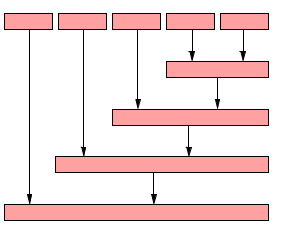
\includegraphics[width=0.6\textwidth]{./images/combinacionsascan.png}
    \caption{Arreglo de sufijos de un texto $T$ formado por la combinación de arreglos de sufijos de los bloques del texto $T$. }
    \label{fig:comb1}
\end{figure}

Se aprecia en la imagen que los bloques de \textit{suffix array} se van combinando desde el final y de manera singular, donde cada uno de ellos se va acoplando con el bloque combinado que dará como resultado al arreglo de sufijos completo para el texto $T$.

Para explicar cómo se realiza la combinación se asumirá que se tiene un string \texttt{T[0,...,n-1]} de tamaño $n$. El texto se divide en bloques de tamaño $m$, donde $m$ es elegido de tal manera que cada una de las estructuras creadas puedan ajustarse según la memoria RAM de tamaño $M$ y no sobrepasarla ($m<M$). Los bloques se procesan comenzando desde el final del texto. Suponer que hasta ahora se ha procesado \texttt{Z = T[i,...,n-1]} y a partir de ese bloque de texto se ha construído el arreglo de sufijos \texttt{SA\textsubscript{Z}}. Luego se procede a construir el arreglo de sufijos \texttt{SA\textsubscript{Y}} del bloque de texto \texttt{Y = T[i-m,...,i-1]} y combinarlo con \texttt{SA\textsubscript{Z}} para formar \texttt{SA\textsubscript{YZ}}. De manera muy general la combinación sigue 2 pasos (ver Figura \ref{fig:comb2}).

El primer paso es comparar el \textit{suffix array} de $Y$ con el texto $Z$ para formar el arreglo \texttt{gap\textsubscript{Y}} que permitirá realizar el segundo paso que es ubicar aquellos sufijos que se ubican entre \texttt{SA\textsubscript{Z}[i]} y \texttt{SA\textsubscript{Z}[i+1]} y realizar la combinación.

Como son bastantes combinaciones a realizar, la complejidad de lectura y escritura en los archivos (\textit{I/O complexity}) y bloques que se forman va por un orden proporcional de $O$($\frac{n^{2}}{M}$) y un tiempo cuya complejidad va por el orden de 0($\frac{n^{2}}{M} \log (2 + \frac{\log \rho}{\log n})$). Como se trabajará con este tipo de algoritmo para el problema de la memoria, se dará mayor detalle de su implementación en el capítulo siguiente (``Implementación'').

\begin{figure}[h]
    \centering
    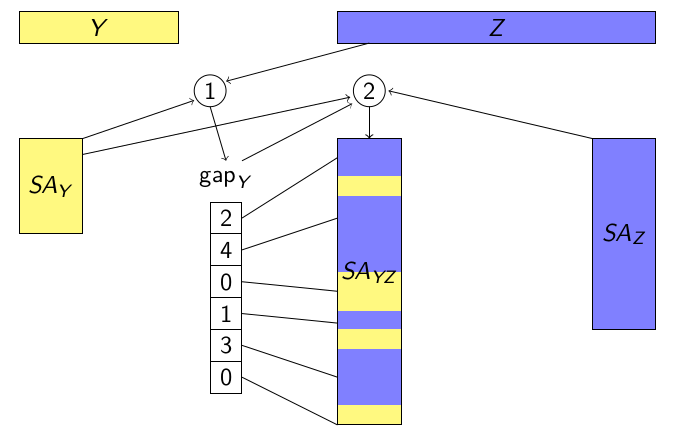
\includegraphics[width=0.8\textwidth]{./images/combinacion2bloques.png}
    \caption{Combinación de 2 arreglos de sufijos que fueron creados de los fragmentos de texto $Y$ y $Z$.}
    \label{fig:comb2}
\end{figure}

\subsection{External Memory LCP Array}

El arreglo de sufijos, en conjunto con su arreglo LCP son la base de soluciones de diversas aplicaciones \cite{aplicacion}. Por consiguiente, cuando comenzó a surgir la implementación del \textit{suffix array} en memoria externa entró a ser materia de investigación la búsqueda de la construcción de un arreglo en LCP también en memoria externa.

Como antes se mencionó, una manera optima de construir el arreglo LCP de un texto $T$ es implementando previamente el arreglo de sufijos del texto $T$ y utilizar este arreglo recien obtenido como \textit{input} para construir el arreglo LCP. Kasai \cite{kasai} fue quien pudo llevar esta idea a una implementación en memoria RAM (memoria interna) pero no fue hasta que Juha Kärkkäinen y Dominik Kempa \cite{lcpscan} pudieron desarrollar una implementación de un arreglo LCP en memoria externa usando como \textit{input} el arreglo de sufijos construido en memoria externa.

Según lo más reciente investigado \cite{emsparse} y para dar un ejemplo sencillo, para obtener el arreglo LCP en memoria externa, se tiene el siguiente texto o string \texttt{T} de tamaño $n$ (\texttt{T} = \texttt{T[0,...,n-1]} = \texttt{T[0]T[1]...T[n-1]}). A partir de este texto se obtiene su arreglo de sufijos \texttt{SA[0,...,n-1]} que es el arreglo ordenado de todos los sufijos del texto $T$. Entonces lo que se quiere obtener para todo $i$ donde $0 \leq i < n$ es el arreglo \texttt{LCP[0,...,n-1]} (el valor de \texttt{LCP[0]} es indefinido) donde \texttt{LCP[i]} = \textit{lcp(\texttt{SA[i]},\texttt{SA[i-1]})}, donde \textit{lcp(j,k)} es la longitud del prefijo común más largo entre el sufijo $j$ y $k$.

Para lograr esto se definen 2 nuevos arreglos, el \textit{arreglo $\Phi$} que consiste en que si se tiene \texttt{j = SA[i]}, entonces se cumple que \texttt{$\Phi$[j] = SA[i-1]} para todo $j$ donde $1 \leq j \leq n$. En otras palabras el sufijo $\Phi$[i] es el predecesor lexicográfico inmediato del sufijo $i$ y por lo tanto \texttt{SA[n-k] = $\Phi_{k}$[SA[n]]} $\forall$ $k$ $\in$ [0,...,n].

El segundo arreglo a definir es conocido como el \textit{arreglo LCP permutado} \texttt{PLCP[0,...,n-1]} es el arreglo LCP permutado desde el orden lexicográfico hacia el orden del texto, es decir, \texttt{PLCP[SA[j]] = LCP[j]} para todo $j$ donde $1 \leq j \leq n$. Por consiguiente \texttt{PLCP[i]} = \textit{lcp(\texttt{i},\texttt{$\Phi$[i]})} $\forall$ $i$ $\in$ [0,...,n-1]. Se considerará un ejemplo con el string \texttt{T = babaabbabbab\$}:

\begin{table}[h]
\centering
\label{my-label12}
\begin{tabular}{|r|ccccccccccccc|}
\hline
\textit{i}  & \multicolumn{1}{c|}{0} & \multicolumn{1}{c|}{1} & \multicolumn{1}{c|}{2} & \multicolumn{1}{c|}{3} & \multicolumn{1}{c|}{4} & \multicolumn{1}{c|}{5} & \multicolumn{1}{c|}{6} & \multicolumn{1}{c|}{7} & \multicolumn{1}{c|}{8} & \multicolumn{1}{c|}{9} & \multicolumn{1}{c|}{10} & \multicolumn{1}{c|}{11} & 12 \\ \hline
T{[}i{]}    & b                      & a                      & b                      & a                      & a                      & b                      & b                      & a                      & b                      & b                      & a                       & b                       & \$  \\
SA{[}i{]}   & 12                     & 3                      & 10                     & 1                      & 7                      & 4                      & 11                     & 2                      & 9                      & 0                      & 6                       & 8                       & 5  \\
$\Phi${[}i{]}  & 9                      & 10                     & 11                     & 12                     & 7                      & 8                      & 0                      & 1                      & 6                      & 2                      & 3                       & 4                       & -  \\
LCP{[}i{]}  & -                      & 0                      & 1                      & 2                      & 2                      & 5                      & 0                      & 1                      & 2                      & 3                      & 3                       & 1                       & 4  \\
PLCP{[}i{]} & 3                      & 2                      & 1                      & 0                      & 5                      & 4                      & 3                      & 2                      & 1                      & 2                      & 1                       & 0                       & -  \\ \hline
\end{tabular}
\caption{Texto \texttt{T = babaabbabbab\$} con su respectivos \texttt{SA[i]}, \texttt{$\Phi$[i]}, \texttt{LCP[i]} y \texttt{PLCP[i]}.}
\end{table}

Por ende los pasos generales para obtener el arreglo LCP en memoria externa tomando como entradas el texto $T$ y el \textit{suffix array} SA (obtenido también por memoria externa) son los siguientes:

\begin{enumerate}

\item Calcular $\Phi$ desde el SA obtenido previamente, si se da el caso se particiona el texto en bloques que se puedan ubicar en la memoria RAM, .
\item Calcular el arreglo PLCP usando el arreglo $\Phi$ y el texto $T$ como base.
\item Calcular el arreglo LCP usando el arreglo PLCP obtenido, acá el texto se particiona en medio-segmentos (\textit{half-segments}) de tal manera que 2 medio-segmentos puedan ser colocados en la memoria RAM.

\end{enumerate}

Se obviarán por ahora detalles mayores de la explicación del funcionamiento de este algoritmo, ya que será analizado y profundizado en el capítulo ``Implementación'' cuando se use este algoritmo para obtener parte de los resultados de la memoria con la base de datos TrEMBL.

\subsection{Transformación de Burrows-Wheeler}

La transformación de Burrows-Wheeler \cite{bwt}, (abreviatura \textit{BWT} del inglés \textit{Burrows–Wheeler transform}, también conocida como compresión por ordenación de bloques), es un algoritmo usado en técnicas de compresión de datos. Fue inventado por Michael Burrows y David Wheeler en 1994 mientras trabajaban en el \textit{DEC Systems Research Center} en Palo Alto, California. Esta transformación consiste en que se toma un trozo de texto $T$ y se le realizan todas las rotaciones posibles, para luego ordenarlas de manera lexicográfica, obteniendo como salida la última columna ubicada en la derecha de la matriz generada (ver Figura \ref{fig:comb3}).

La aplicación más importante que tiene esta transformación es la de compresión de datos (usada por ejemplo la usada en la Alineación de Bowtie \cite{bowtie}) y también mantiene correlación con el arreglo de sufijos, el cual será utilizado en el \textit{External Memory Suffix Array} para este trabajo (en el capítulo ``Implementación'' se detallará cúal es la función de esta transformación).

\newpage

\begin{figure}[h]
    \centering
    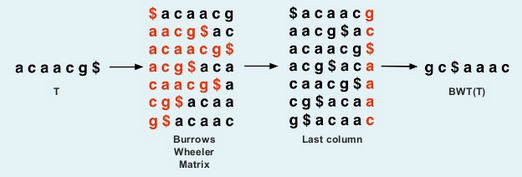
\includegraphics[width=0.6\textwidth]{./images/bwtejemplo.png}
    \caption{Ejemplo de la transformación de Burrows-Wheeler para la cadena acaacg\$.}
    \label{fig:comb3}
\end{figure}
%archivo propuesta
\chapter{Implementación}

\section{Propuesta considerada}

Examinando las técnicas anteriormente revisadas, se llega al punto de que lo más factible es trabajar con las cadenas de secuencias utilizando un arreglo que las encadene una a una. Recordando los objetivos que se tienen para esta memoria, estas son:

\begin{enumerate}
\item Obtener la cantidad total de diferentes residuos de aminoácidos de tamaño $k =$ 1 hasta 50 que existen para las bases de datos de UniProt-SwissProt y UniProt-TrEMBL.
\item Encontrar para cada caso anterior cuáles son los residuos de aminoácidos que más se repiten.
\end{enumerate}

Para realizar la primera tarea, será necesario construir un \textit{suffix array} el cual será la base del arreglo LCP para realizar este objetivo. Considerando un ejemplo sencillo como la palabra BANANA\$:

\begin{table}[H]
	\centering
	\begin{tabular}{c l}
		\textit{\textbf{SA[]}} & \textit{\textbf{sufijo}}\\
		6 & \$\\
		5 & A\$\\
		3 & ANA\$\\
		1 & ANANA\$\\
		0 & BANANA\$\\
		4 & NA\$\\
		2 & NANA\$\\
	\end{tabular}
\end{table}

Se puede apreciar que los números asociados a cada sufijo ya están ordenados como si fuera un arreglo de sufijos. Es posible obtener la cantidad total de diferentes substrings que componen esta palabra utilizando el arreglo LCP de la siguiente forma. Introduciendo los 2 siguientes conceptos:

{\it{length}}('X') = Largo de caracteres de la palabra 'X'.\\
{\it{LCP}}('Y','Z') = Prefijo más largo en común ({\it{Longest Common Prefix}}) entre los substrings 'Y' y 'Z'.

Y partiendo según el orden alfabético dado anteriormente, se hace el siguiente ejercicio:

Largo primer sufijo ordenado ('\$') = 1 = $var$\\
Comienzo de pares de sufijos:
\begin{enumerate}
	\item ('\$','A\$'): $var +=$ {\it{length}}('\$A') - {\it{LCP}}('\$','\$A')\\
	$var=var+2-0 =>  1+2=3$

	\item ('A\$','ANA\$'): $var +=$ {\it{length}}('ANA\$') - {\it{LCP}}('A\$','ANA\$')\\
	$var=var+4-1 =>  3+3=6$
	
	\item ('ANA\$','ANANA\$'): $var +=$ {\it{length}}('ANANA\$') - {\it{LCP}}('ANA\$','ANANA\$')\\
	$var=var+6-3 =>  6+3=9$
	
	\item ('ANANA\$','BANANA\$'): $var +=$ {\it{length}}('BANANA\$') - {\it{LCP}}('ANANA\$','BANANA\$')\\
	$var=var+7-0 =>  9+7=16$
	
	\item ('BANANA\$','NA\$'): $var +=$ {\it{length}}('NA\$') - {\it{LCP}}('BANANA\$','NA\$')\\
	$var=var+3-0 =>  16+3=19$
	
	\item ('NA\$','NANA\$'): $var +=$ {\it{length}}('NANA\$') - {\it{LCP}}('NA\$','NANA\$')\\
	$var=var+5-2 =>  19+3=22$
	
\end{enumerate}

Cantidad de diferentes substrings que hay en BANANA\$: 22.

Lo que se hace en este caso es crear una variable y guardar la longitud del primer sufijo del SA (en este caso \$) para luego realizar una comparación entre los sufijos consecutivos $i$ y $j$ adicionando en cada caso a la variable las longitudes respectivas de los sufijos $j$, y además \textbf{se le resta el prefijo común más largo entre estos sufijos consecutivos}:

\begin{table}[H]
	\centering
	\label{propuesta-1}
	\begin{tabular}{c c l}
		\textit{\textbf{SA[]}} & \textit{\textbf{LCP[]}} &\textit{\textbf{sufijo}}\\
		6 & 0 & \$\\
		5 & 0 & A\$\\
		3 & 1 & ANA\$\\
		1 & 3 & ANANA\$\\
		0 & 0 & BANANA\$\\
		4 & 0 & NA\$\\
		2 & 2 & NANA\$\\
	\end{tabular}
\caption{SA y arreglo LCP de la palabra BANANA\$}
\end{table}

Entonces, particularizando el problema, ¿cómo sería posible obtener la cantidad total de diferentes substrings de un determinado tamaño? La clave está en el \textbf{arreglo LCP} obtenido, el cual se puede utilizar desde 2 perspectivas para realizar esta tarea.

\subsection{Restando la cantidad máxima posible de diferentes substrings}

Primero que todo hay que considerar la cantidad potencial máxima de diferentes substrings de tamaño $k$ que se pueden obtener (la fórmula es $n-k+1$ donde $n$ es el largo de la palabra) y luego se recorre el arreglo LCP utilizando el valor de $k$ como un comparador.
Por ejemplo, de la palabra BANANA\$ a simple vista se sabe que los diferentes substrings de tamaño 1 que se encuentran son 4, que son A, B, N y \$. Usando la fórmula mencionada en el párrafo anterior se tiene que $7-1+1=7$ es la cantidad máxima de substrings de tamaño 1 de esta palabra. Recorriendo el arreglo LCP es necesario encontrar aquellos valores que sean \textbf{mayores o iguales que $k$} para restarlos a la cantidad máxima de diferentes substrings, porque ese valor indica en el arreglo de sufijos si determinado sufijo se \textbf{repite más de una vez}, por consiguiente esto indica que disminuye en una unidad la cantidad total de diferentes substrings de determinado tamaño. Aplicando en el caso anterior:

Máxima cantidad de diferentes substrings de tamaño 1 para BANANA\$: $DS = 7$

$a)$ $LCP[0]=0 =>$ DS se mantiene $=> DS=7$\\
$b)$ $LCP[1]=0 =>$ DS se mantiene $=> DS=7$\\ 
$c)$ $LCP[2]=1 =>$ $DS=7-1=6$\\ 
$d)$ $LCP[3]=3 =>$ $DS=6-1=5$\\
$e)$ $LCP[4]=0 =>$ DS se mantiene $=> DS=5$\\
$f)$ $LCP[5]=0 =>$ DS se mantiene $=> DS=5$\\
$g)$ $LCP[6]=2 =>$ $DS=5-1=4$ 

Diferentes substrings en total de tamaño 1 en la palabra BANANA\$: 4.

Para los tamaños 2 hasta 7 (palabra completa) los diferentes substrings encontrados son los siguientes:\\

\begin{table}[H]
\centering
\label{propuesta-12}
\begin{tabular}{|c|c|c|}
\hline
Tamaño 2     & Tamaño 3      &  Tamaño 4   \\
Substrings totales: 6      &  Substrings totales: 5    & Substrings totales: 4   \\
Elementos LCP $\geq$ 2: 2       & Elementos LCP $\geq$ 3: 1       & Elementos LCP $\geq$ 4: 0      \\
DS de tamaño 2: $6-2 = 4$      & DS de tamaño 3: $5-1 = 4$          & DS de tamaño 4: $4-0 = 4$            \\ \hline
Tamaño 5     & Tamaño 6      &  Tamaño 7   \\
Substrings totales: 3      &  Substrings totales: 2    & Substrings totales: 1   \\
Elementos LCP $\geq$ 5: 0       & Elementos LCP $\geq$ 6: 0       & Elementos LCP $\geq$ 7: 0      \\
DS de tamaño 5: $3-0 = 3$      & DS de tamaño 6: $2-0 = 2$          & DS de tamaño 7: $1-0 = 1$            \\ \hline
\end{tabular}
\end{table}

Sumando los DS encontrados entre los tamaños 1 hasta 7 el valor es de $4+4+4+4+3+2+1=22$, obteniendo el mismo valor de antes.

\subsection{Aumentando la cantidad de diferentes substrings desde 0 considerando determinados tamaños de LCPs consecutivos}

Esta segunda perspectiva considera recorrer el arreglo LCP con una pequeña variación, la que sería mover el primer elemento del arreglo (que siempre será 0) y dejarlo en la última posición desde izquierda a derecha:

\begin{table}[h]
\centering
\label{propuesta-2}
\begin{tabular}{|l|l|l|l|l|l|l|l|l|l|l|l|l|l|l|}
\cline{1-7} \cline{9-15}
0 & 0 & 1 & 3 & 0 & 0 & 2 & -\textgreater & 0 & 1 & 3 & 0 & 0 & 2 & 0 \\ \cline{1-7} \cline{9-15} 
\end{tabular}
\caption{Arreglo LCP (tabla izquierda) mueve su primer elemento (0) hacia la última posición (tabla derecha).}
\end{table}

El motivo de esto es identificar el prefijo común más largo entre los 2 sufijos consecutivos entre los sufijos $x$ e $y$ considerando al {\textbf{primero o sufijo \textit{x}}} como el sufijo de referencia:

\begin{table}[H]
	\centering
	\label{propuesta-21}
	\begin{tabular}{c c l}
		\textit{\textbf{SA[]}} & \textit{\textbf{LCP[]}} &\textit{\textbf{sufijo}}\\
		6 & 0 & \$\\
		5 & 1 & A\$\\
		3 & 3 & ANA\$\\
		1 & 0 & ANANA\$\\
		0 & 0 & BANANA\$\\
		4 & 2 & NA\$\\
		2 & 0 & NANA\$\\
	\end{tabular}
\caption{SA y arreglo LCP modificado de la palabra BANANA\$}
\end{table}

Para que sea más entendible, el último valor del arreglo LCP modificado es 0 ya que NANA\$ es el último sufijo, y no tiene un sufijo posterior con el cual compararse.

En esta ocasión no se considerará la máxima cantidad de diferentes substrings de tamaño $k$ ($n-k+1$) ya que todo se obtendrá del \textit{suffix array} y de su arreglo LCP correspondiente, y el realizar esta modificación en el arreglo LCP permitirá lograr el segundo objetivo para este trabajo, que es el de encontrar a los conjuntos de péptidos que más se repiten para un determinado tamaño. Se puede ejemplificar esto con la búsqueda de los diferentes substrings de tamaño 3 en la palabra BANANA\$:

Se inicializa con $DS = 0$.

a) $LCP[0]=0 =>$ se mantiene $=> DS=0$ ya que el tamaño del sufijo es menor a 3 ($SA[0]=$ \$).\\
b) $LCP[1]=1 =>$ se mantiene $=> DS=0$ ya que ocurre el mismo fenómeno de antes ($SA[1]=$ A\$).\\ 
c) $LCP[2]=3 => SA[2] =$ ANA\$, este sufijo con su siguiente sufijo consecutivo tiene como \textit{longest common prefix} a ANA, por lo tanto se sabe que ANA se repite al menos 2 veces en la palabra; por ahora se seguirá dejando $DS = 0$.

Aquí viene la premisa del LCP consecutivo, ya que si el siguiente valor del arreglo LCP (para este caso $LCP[3]$) fuera mayor o igual que 3, entonces se tendría una nueva repetición del prefijo ANA, por lo tanto ahora serían 3 las veces que este prefijo estaría repetido en la palabra. Entendiéndolo de manera más formal, se tendrían \textbf{$l$ valores consecutivos desde la posición $s$ del arreglo LCP que serían mayores que $k$ (que para este caso es 3)}, entregando un total de $l+1$ repeticiones del sufijo $SA[s]$ de tamaño $k$. En caso contrario (valor del arreglo LCP menor que 3), se acabarían las repeticiones de determinado sufijo y se agrega una unidad al total de diferentes substrings encontrados.

d) $LCP[3]=0 =>$ Aquí el valor es menor que 3, por lo tanto $DS=0+1=1$ y se tiene que ``ANA'' se repite 2 veces.\\
e) $LCP[4]=0 =>$ Tamaño $SA[4] = 7$, $SA[4,3] =$ BAN, por lo tanto $DS=1+1=2$.\\
f) $LCP[5]=2 =>$ Tamaño $SA[5] = 3$, $SA[5,3] =$ NA\$, por lo tanto $DS=2+1=3$.\\
g) $LCP[6]=0 =>$ Tamaño $SA[6] = 5$, $SA[6,3] =$ NAN, por lo tanto $DS=3+1=4$.\\

Por consiguiente, se tiene que los diferentes substrings de tamaño 3 para la palabra BANANA\$ son 4, ANA que se repite 2 veces, BAN, NA\$ y NAN, que se repiten solo una vez. Sumando estas cantidades se tiene un valor de 5, que es el \textbf{número total de substrings de tamaño 3} ($n-k+1$).

Por ende para la realización del algoritmo se utilizará esta segunda premisa, considerando las restricciones pertinentes para este trabajo, no obstante, es necesario encontrar alguna estructura que permita guardar aquellos residuos que más se repitan para cumplir con el objetivo completo de este trabajo, este punto se explicará en la siguiente sección.

\section{Cola de prioridad \textit{(priority queue)}}

La estructura conocida como \textit{priority queue} \cite{queues} es un tipo de estructura contenedora implementada en C++ \cite{tutorial} similar a una lista, vector o arreglo, con su característica principal que al único elemento que se puede acceder es aquel que \textbf{sí o solo si tenga la prioridad o valor más alto que los demás elementos}. En otras palabras, se pueden ir agregando varios elementos a esta estructura y dependiendo del valor que tengan el elemento con la prioridad más alta puede variar, de tal forma que extrayendo todos los elementos del \textit{priority queue} estos van siendo removidos desde aquel que tenga la prioridad más alta hasta llegar al elemento con la prioridad más baja. Este contexto es similar a un \textit{heap} \cite{tutorial}, donde los elementos pueden ser insertados en cualquier momento, y solamente el elemento con el máximo valor \textit{(max heap)} puede ser obtenido (el elemento en la primera posición en el \textit{priority queue}).

Se puede ejemplificar de la siguiente forma, se crea un \textit{priority queue} de enteros y se insertan los valores: 14, 8, 35, 11 y 27.

\begin{figure}[h]
\centering
\begin{tikzpicture}[sibling distance=5em,
  every node/.style = {shape=rectangle, rounded corners,
    draw, align=center,
    top color=white, bottom color=blue!20}]]
  \node {35}
    child { node {14} }
    child { node {8} }
    child { node {11} }
    child { node {27} };
\end{tikzpicture}
\caption{Grafo de muestra del formato de un \textit{priority queue}.}
\end{figure}

El número 35 es el valor más alto y el que tiene la mayor prioridad, por lo tanto es el elemento al que se puede acceder. Ahora si ese valor se extrae, el \textit{priority queue} se reordena y queda de la siguiente forma:

\begin{figure}[h]
\centering
\begin{tikzpicture}[sibling distance=5em,
  every node/.style = {shape=rectangle, rounded corners,
    draw, align=center,
    top color=white, bottom color=blue!20}]]
  \node {27}
    child { node {14} }
    child { node {8} }
    child { node {11} };
\end{tikzpicture}
\caption{El \textit{priority queue} con el número 35 extraído.}
\end{figure}

En este caso el segundo valor más alto del \textit{priority queue} original (el número 27) es el nuevo elemento con la prioridad mayor y al que se puede acceder.

Ahora si se desea agregar un nuevo número a este arreglo, por ejemplo el 15, ocurre lo siguiente:

\begin{figure}[h]
\centering
\begin{tikzpicture}[sibling distance=5em,
  every node/.style = {shape=rectangle, rounded corners,
    draw, align=center,
    top color=white, bottom color=blue!20}]]
  \node {27}
    child { node {14} }
    child { node {8} }
    child { node {11} }
    child { node {15} };
\end{tikzpicture}
\caption{El \textit{priority queue} con el número 15 agregado.}
\end{figure}

Como el número 15 es menor que 27, se mantiene este número como la mayor prioridad.

\subsection{Algunos comandos de C++ para el \textit{priority queue}}

En C++ se define como \texttt{priority\_queue<int>} ``nombre\_arreglo'' para guardar valores enteros, para este caso se definirá \texttt{mypq} como el nombre de ejemplo para esta estructura. Las operaciones más importantes que se pueden realizar para este tipo de estructura son las siguientes:

\begin{enumerate}

\item \texttt{mypq.push(n)}: Inserta el número $n$ en el \textit{priority queue}.
\item \texttt{mypq.top()}: Retorna el valor con mayor prioridad del \textit{priority queue}.
\item \texttt{mypq.pop()}: Remueve el valor con mayor prioridad del \textit{priority queue}, disminuyendo el tamaño de esta estructura en uno.
\item \texttt{mypq.empty()}: Retorna si el \textit{priority queue} está vacío.

\end{enumerate}

A partir de estas operaciones es posible manipular el \textit{priority queue} de manera más fácil, de tal manera que se usará esta estructura para guardar y obtener aquellos residuos de proteínas que más se repiten, sin embargo, para resolver el problema descrito será necesario guardar en este arreglo especial tanto el fragmento del péptido como la cantidad de repeticiones que posea, detalle que será visto en la sección de implementación.

\section{Restricciones para la propuesta}

Primero que todo, se extraerán las secuencias de polipéptidos de los archivos .fasta y se alinearán en una \textbf{única gran cadena} donde cada secuencia estará unida por un signo \$, con esto será posible identificar en los arreglos si cierto sufijo está compuesto por este signo o no, de esa forma descartarlo dentro de los diferentes residuos de aminoácidos que se cuentan:

\begin{table}[h]
\centering
\label{propuesta-22}
\begin{tabular}{c}
$\ldots$MPSTLQVLAKKVLKENDHISR\$EYHILKCWHEAPIILCFNGSKQM$\ldots$\\ 
\end{tabular}
\caption{2 secuencias enlazadas en una cadena general utilizando el signo \$ como unión.}
\end{table}

Para esta cadena grande (de largo $m$), el arreglo de sufijos y el arreglo LCP tendrán tamaño $m$, por lo cual para determinar los diferentes substrings de tamaño $k$ y aquellos substrings que más se repiten se debe recorrer el arreglo LCP completo, considerando:

\begin{enumerate}
\item Si el largo del sufijo es mayor o igual a $k$, entonces el arreglo LCP puede ser analizado, en caso contrario se omite y se continúa al siguiente valor del arreglo LCP.
\item Si el prefijo del sufijo revisado \textbf{solamente esté compuesto por los 20 aminoácidos conocidos} \cite{biomolecula}. Otros aminoácidos que no han sido definidos, como B, J, O, U o X serán omitidos para este problema (si son parte del substring del sufijo revisado, se omitirá y se continuará al arreglo LCP siguiente) y considerados como prohibidos \cite{aminoacids}. El signo \$ también será incluído a este grupo de carácteres prohibidos.
\end{enumerate}

Con respecto a esto es posible obtener los substrings diferentes y la cantidad de repeticiones que posee cada uno de estos, para posteriormente guardarlos en algun tipo de lista o vector. El problema es tratar de acceder a aquellos substrings que más se repiten, detalle que se verá en la siguiente sección.

\section{Algoritmo desarrollado}

Para la obtención de los diferentes substrings se realizó un código implementado en lenguaje C++ \cite{tutorial} siguiendo varios puntos, en primera instancia para la base de datos de SwissProt y TrEMBL se realizó una extracción previa de datos.

El archivo ``uniprot\_sprot.fasta'' está compuesto por 555426 proteínas con un peso total de 268 MB, mientras que el ``uniprot\_trembl.fasta'' está compuesto por 88032926 proteínas con un peso de 40 GB. Para ambos archivos la construcción del arreglo de sufijos y el arreglo LCP serán diferentes pero recibirán la misma cadena enlazada, cuya construcción será explicada en la siguiente sección.

\subsection{Extracción de proteínas desde el archivo .fasta}

EL archivo \textbf{.fasta} entrega cada polipéptido con un código o ID (que comienza con un $>$), a continuación en la misma línea se tiene al nombre taxativo de la proteína, y en la línea siguiente viene la cadena como tal, para luego repetir el proceso:

\begin{figure}[h]
    \centering
    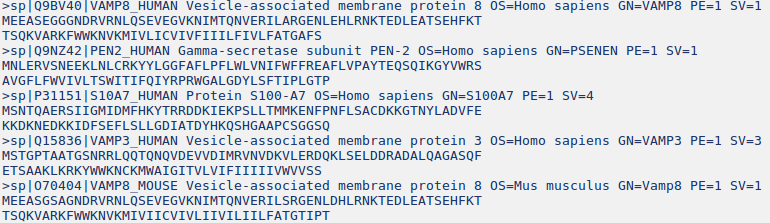
\includegraphics[width=0.9\textwidth]{./images/fastadefecto2.png}
    \caption{Archivo \textbf{.fasta} por defecto con varias proteínas}
    \label{fig:image5}
\end{figure}

Para extraer las cadenas se implementó el siguiente código en C++:

\begin{lstlisting}[language=C++, caption=Creación de cadena de proteínas]
ifstream fin("uniprot_sprot.fasta"); //abrir archivo base
if(!fin){
	cerr << "Couldn't open the input file!";
	return(1);
}
ofstream outputfile; //crear archivo destino de cadena
outputfile.open("substrings.txt"); //definir nombre de archivo a crear
string line; 
int cantidad_ss = 1;

getline(fin, line); 
getline(fin, line); //tomar secuencia (1)

while(fin){
	if(line[0] == '>'){ // revisar primer elemento del string (2)
		outputfile << "$";
		cantidad_ss = cantidad_ss + 1;
	}
	else{
		outputfile << line;
	}
getline(fin, line); // continuar con la siguiente linea (3)
}

outputfile.close();
\end{lstlisting}

Lo que hace este código es crear un nuevo archivo ``substrings.txt'' en la variable \textbf{outputfile} donde se guardará la cadena de proteínas. Con \textit{getline} se lee la primera ĺinea del archivo .fasta que está guardada en la variable \textbf{fin}, e inmediatamente después se llama nuevamente a \textit{getline} para leer la segunda línea del archivo .fasta, que es \textbf{una secuencia o parte de ella} (1). Luego se condiciona a realizar una de las 2 tareas siempre y cuando el archivo .fasta no se haya leído completamente: 

\begin{enumerate}
\item Si el primer elemento de la línea leída del archivo .fasta es $>$, significa que se llegó al final de una secuencia, por lo tanto es el comienzo de la siguiente (es la linea de definición de la proteína), en ese caso se le agrega el signo \$ al archivo destino como separador (2). 
\item En caso contrario, se le agrega directamente la línea completa al archivo destino, ya que esta línea solamente está compuesta por \textbf{la secuencia en sí}.
\end{enumerate}

Finalmente se vuelve a llamar a \textit{getline} para continuar con la siguiente línea del archivo .fasta (3).

En resumen el formato del nuevo archivo ``substrings.txt'' es una sola línea que tiene concatenada todas las proteínas:

\begin{table}[h]
\centering
\label{propuesta-23}
\begin{tabular}{c}
TSCPGGNHPVCCSTDLCNK\$MKTL$\ldots$SDLT\$LKCNKLVPLFYKTCP\\ 
\end{tabular}
\caption{Ejemplo de cadena encontrada en el archivo destino}
\end{table}

Teniendo esta gran línea ya se puede construir el arreglo de sufijos y el arreglo LCP. Considerar como dato relevante que guardando esta cadena en una variable tipo \textit{string} cada caracter ocupa el tamaño de 1 byte de capacidad \cite{manipulatingstrings}, y esto determinará de qué manera se construirán los arreglos para la solución de este problema.

Por defecto se tiene que el tamaño de UniProt-SwissProt es de 268 MB y su cadena de proteínas tiene un peso de 199 MB, mientras que para UniProt-TrEMBL su tamaño por defecto es de 40 GB y su cadena de proteínas posee un peso de 30 GB, si se tiene en consideración que para guardar la cadena en una variable esta se almacena en la memoria RAM del ordenador. En primera instancia no hay problema con la base de datos de SwissProt ya que el espacio ocupado es suficiente si se trabaja en un computador normal (si se guardan los arreglos en una variable tipo \textit{vector}, cada elemento del vector pesa 4 bytes), pero para la cadena creada en función de UniProt-TrEMBL parece ser más complejo, ya que el string para almacenar la cadena requeriría 30 GB de memoria RAM, inclusive ocupando un servidor con 50 GB de capacidad de RAM sería inviable construir los arreglos (en cálculos sencillos se necesitaría de una RAM de al menos 300 GB para realizar esta tarea). Una posible solución para esto se revisará más adelante en la implementación para la base de datos UniProt-TrEMBL.

\subsection{Implementación solución para base de datos UniProt-SwissProt}

Para la implementación del algoritmo se trabajó por medio del lenguaje C++ en base al algoritmo de Kasai \cite{kasaimethod}, \cite{kasai} para obtener el arreglo LCP en base al arreglo de sufijos. Antes que nada se define una estructura y una función comparativa que serán de soporte para la construcción del arreglo de sufijos:

\begin{lstlisting}[language=C++, caption=Definición previa de estructuras para construir el arreglo de sufijos.]
//  Struct para guardar la informacion de un sufijo
struct suffix
{
	int index; // Guardar el indice original
	int rank[2]; // Guarda los ranks y el rank pair siguiente
};

// Una funcion comparativa usada por sort () para comparar 2 sufijos
// Compara 2 pares, y retorna 1 si el primer par es mas pequeno
int cmp(struct suffix a, struct suffix b)
{
	return (a.rank[0] == b.rank[0])? (a.rank[1] < b.rank[1] ?1: 0):
		(a.rank[0] < b.rank[0] ?1: 0);
}
\end{lstlisting}

\textit{suffix} es una estructura que sirve para almacenar el índice original de determinado sufijo y los \textit{rank} donde se guardan los sufijos y su sufijo siguiente como pares. La función \textit{cmp} es usada para comparar entre los valores de los \textit{rank} entre 2 sufijos, y retorna 1 si el primer par es más pequeño, si son igual se continua la comparación con el siguiente par, y es el comparador base que será usado por la función \textit{sort} más adelante.

\subsubsection{Arreglo de sufijos implementado}

Ahora se procederá a explicar la función principal que toma un string ``txt'' de tamaño n como entrada, y que construye y retorna el arreglo de sufijos para el string dado. Será explicado en secciones que fueron numerados en parte del código (con un //(número)) para aprovechar en mejor manera el formato de este documento:

\begin{lstlisting}[language=C++, caption=Función principal arreglo de sufijos (1)]
vector<int> buildSuffixArray(string txt, int n){

	struct suffix *suffixes = new struct suffix [n]; //(1)
	for (int i = 0; i < n; i++){
		suffixes[i].index = i;
		suffixes[i].rank[0] = txt[i] - 'a';
		suffixes[i].rank[1] = ((i+1) < n)? (txt[i + 1] - 'a'): -1;
	}
	sort(suffixes, suffixes+n, cmp); 
	int *ind = new int [n]; //(2)
	for (int k = 4; k < 2*n; k = k*2){
		int rank = 0;
		int prev_rank = suffixes[0].rank[0];
		suffixes[0].rank[0] = rank;
		ind[suffixes[0].index] = 0;//(3)
		for (int i = 1; i < n; i++){
			if (suffixes[i].rank[0] == prev_rank && 
			  suffixes[i].rank[1] == suffixes[i-1].rank[1]){ \\(a)
				prev_rank = suffixes[i].rank[0];
				suffixes[i].rank[0] = rank;
			}
			else
			{
				prev_rank = suffixes[i].rank[0]; \\(b)
				suffixes[i].rank[0] = ++rank;
			}
			ind[suffixes[i].index] = i;
		}
		for (int i = 0; i < n; i++){
			int nextindex = suffixes[i].index + k/2;
			suffixes[i].rank[1] = (nextindex < n)?
			    suffixes[ind[nextindex]].rank[0]: -1;
		}
		sort(suffixes, suffixes+n, cmp);//(4)
	}
	vector<int>suffixArr;
	for (int i = 0; i < n; i++){
        suffixArr.push_back(suffixes[i].index);
    }//(5)
	delete [] ind;
	delete [] suffixes;
	return suffixArr;//(6)
}

\end{lstlisting}

En \textbf{(1)} se crea un estructura que almacena sufijos y sus indices (\textit{suffixes}), que se alojará en memoria dinámica (operador new), esta estructura es necesaria para ordenar los sufijos de manera alfabética y mantener sus antiguos índices mientras se ordena. 

Luego con la función \textit{sort} se ordenan los sufijos de acuerdo a sus \textbf{2 primeros caracteres}. Una vez realizado esto de manera posterior se ordenan los sufijos de acuerdo a sus primeros 4 caracteres, luego con sus primeros 8 caracteres y asi sucesivamente hasta $k > 2^{n}$ donde $n$ es el largo del string analizado, para realizar esta tarea se crea un arreglo dinámico \textit{ind} que es necesario para obtener el indice original en la estructura suffixes[] \textbf{(2)}.

En cada una de estas iteraciones se le asigna los valores de \textit{rank} e índice al primer sufijo  \textbf{(3)}, luego se le asigna los \textit{rank} a los siguientes sufijos hasta $n$ siguiendo ciertas reglas:

$a)$ Si el primer \textit{rank} y los siguientes ranks son iguales a aquellos de los sufijos anteriores en el arreglo, asignar el mismo nuevo rank a ese sufijo.\\
$b)$ En caso contrario aumentar el \textit{rank} y asignar.

Después se le asigna el próximo \textit{rank} a cada sufijo para posteriormente ordenar los sufijos según los primeros $k$ caracteres \textbf{(4)}. Se realiza este proceso hasta terminar las iteraciones para la variable $k$.

Finalmente en \textbf{(5)} se crea un vector que permita almacenar los valores obtenidos de los índices ordenados del arreglo \textit{suffixes}. Este vector de enteros \textit{suffixArr} se convertirá en el \textbf{arreglo de sufijos} del string \textit{txt}, luego se borran los arreglos dinámicos \textit{suffixes} e \textit{ind} para desocupar el espacio asignado en memoria RAM.

Posteriormente \textbf{(6)} se retorna el arreglo de sufijos, que permitirá construir el arreglo LCP.

\subsubsection{Arreglo LCP implementado}

La implementación de este arreglo se hizo en base al \textit{suffix array} implementado, siguiendo lo descrito por Kasai \cite{kasaimethod}, \cite{kasai}. El código realizado es el siguiente:

\begin{lstlisting}[language=C++, caption=Función principal arreglo LCP (1)]
vector<int> lcp_str(string txt, vector<int> suffixArr){
	int n = suffixArr.size();
	vector<int> lcp(n, 0);
	vector<int> invSuff(n, 0); \\(1)
	for (int i=0; i < n; i++)
		invSuff[suffixArr[i]] = i;

	int k = 0; \\(2)
	for (int i=0; i<n; i++){
		if (invSuff[i] == n-1){
			k = 0;
			continue; \\(3)
		}
		int j = suffixArr[invSuff[i]+1];\\(4)
		while (i+k<n && j+k<n && txt[i+k]==txt[j+k]) \\(5)
			k++;
		lcp[invSuff[i]] = k; \\(6)
		if (k>0)
			k--;
	}
	return lcp; \\(7)
}

\end{lstlisting}

Lo que se hace en primera instancia es guardar el largo del arreglo, crear un vector para almacenar el arreglo LCP a construir y además crear un arreglo auxiliar $invSuff$ para almacenar el inverso del arreglo de sufijos previamente creado. Por ejemplo si $suffixArr[0]$ es 5, entonces $invSuff[5]$ debiese ser 0. Y esto será usado para obtener el siguiente string del arreglo de sufijos \textbf{(1)}.

Luego se llena con valores el arreglo $invSuff$ y se inicializa una variable para guardar la longitud del LCP del sufijo \textbf{(2)}. A partir de acá comienza a revisar todos los sufijos para asignarles su valor en el arreglo LCP.

Un detalle importante se ubica en \textbf{(3)}, ya que si el sufijo actual está ubicado en la posicion $n-1$, entonces ya no hay un siguiente substring a considerar, por lo tanto el LCP no es definido para este substring y se hace cero. Esto permitirá enfocar la solución del problema aumentando la cantidad de diferentes substrings desde 0 considerando determinados tamaños de LCPs consecutivos.

Posteriormente en la iteración se define una variable $j$ que contiene el índice del siguiente substring a ser considerado para compararlo con el actual substring, es decir, el siguiente string en el arreglo de sufijos \textbf{(4)}. Después la función \textit{while} comienza a revisar el sufijo desde el $k$-ésimo indice donde al menos $k-1$ caracteres serán similares, mientras esta condición se cumpla, $k$ va aumentando \textbf{(5)}.

Posteriormente se asigna el valor del LCP encontrado para el actual sufijo \textbf{(6)}, y $k$ se borra para utilizarlo en la siguiente iteración. Finalmente se retorma el arreglo LCP obtenido \textbf{(7)}.

Con esto se tienen a disposición los 2 arreglos necesarios como base para resolver el problema de la memoria.

\subsubsection{Implementación programa principal}

Ahora se procederá a explicar la implementación cómo se obtuvieron los diferentes substrings totales para cada $k$ entre 1 hasta 50 y la obtención de los residuos que más se repiten para cada caso. En primer lugar cuando la cadena de proteínas fue construída se definió una variable llamada \texttt{cantidad\_ss}, que guarda la cantidad total de proteínas analizadas. Utilizando las implementaciones del arreglo de sufijos y el arreglo LCP ocurre lo siguiente:

\begin{lstlisting}[language=C++, caption=Obtención de los arreglos SA y LCP para la cadena de proteínas.]
ifstream file("substrings.txt");
stringstream buffer;
buffer << file.rdbuf();
string str = buffer.str(); \\(1)

unsigned t0, t1, t2, t3, t4, t5;
t0 = clock();
vector<int>suffixArr = buildSuffixArray(str, str.length());
t1 = clock();
double t12 = (double(t1-t0)/CLOCKS_PER_SEC); \\(2)

t2 = clock();
vector<int>lcp = lcp_str(str, suffixArr);
t3 = clock();
double t23 = (double(t3-t2)/CLOCKS_PER_SEC); \\(3)

ofstream resultados, k_utilizados; \\(4)
resultados.open("resultados_sa_lcp.txt");
resultados << "Construccion SA: " << t12 << " segundos" << endl;
resultados << " \n";
resultados << "Construccion LCP: " << t23 << " segundos" << endl;
resultados << " \n";
resultados << "Total: " << cantidad_ss << " proteinas" << endl; \\(5)
resultados.close();
	
\end{lstlisting}

En primera instancia se debe guardar la cadena de proteínas creada en el archivo ``substrings.txt'' en el string \texttt{str} \textbf{(1)}, para luego construir el arreglo de sufijos \textbf{(2)} que se guarda en el vector \texttt{suffixArr} y el arreglo LCP que se guarda en el vector \texttt{lcp} \textbf{(3)}. En ambos casos se obtienen los tiempos respectivos que demora en construir estos arreglos.

Después se crean 2 variables para crear archivos, en uno se guardarán los tiempos de construcción de los arreglos, y en otro los diferentes substrings para determinados $k$ con sus respectivos residuos que más se repiten \textbf{(4)}. A la primera variable se abre el archivo ``resultados\_sa\_lcp.txt'' y le agregan al archivo los tiempos de construcción de los 2 arreglos \textbf{(5)}, posteriormente este archivo se cierra.

El formato de los arreglos obtenidos es el siguiente:

\begin{table}[h]
\centering
\label{my-label15}
\begin{tabular}{llllllllllllll}
\cline{2-13}
\multicolumn{1}{l|}{Arreglo SA}  & \multicolumn{1}{l|}{...} & \multicolumn{1}{l|}{34} & \multicolumn{1}{l|}{22} & \multicolumn{1}{l|}{15} & \multicolumn{1}{l|}{89} & \multicolumn{1}{l|}{901} & \multicolumn{1}{l|}{1042} & \multicolumn{1}{l|}{45} & \multicolumn{1}{l|}{4} & \multicolumn{1}{l|}{47} & \multicolumn{1}{l|}{59} & \multicolumn{1}{l|}{...} &  \\ \cline{2-13}
                                 &                          &                         &                         &                         &                         &                          &                           &                         &                        &                         &                         &                          &  \\ \cline{2-13}
\multicolumn{1}{l|}{Arreglo LCP} & \multicolumn{1}{l|}{...} & \multicolumn{1}{l|}{2}  & \multicolumn{1}{l|}{0}  & \multicolumn{1}{l|}{21} & \multicolumn{1}{l|}{3}  & \multicolumn{1}{l|}{8}   & \multicolumn{1}{l|}{3}    & \multicolumn{1}{l|}{2}  & \multicolumn{1}{l|}{0} & \multicolumn{1}{l|}{0}  & \multicolumn{1}{l|}{9}  & \multicolumn{1}{l|}{...} &  \\ \cline{2-13}
\end{tabular}
\caption{Formatos de los arreglos SA y LCP}
\end{table}

Recordar que todos los elementos del arreglo de sufijos son diferentes.

Para cada $k$ los arreglos se deben recorrer desde el principio hasta el final, con esto será posible obtener los diferentes residuos de péptidos y los que más se repiten. Esto se implementó de la siguiente forma:

\begin{lstlisting}[language=C++, caption=Obtención de los diferentes substrings de tamaño $k$ y los 20 substrings que más se repiten para la cadena de proteínas.]
int inicio = cantidad_ss - 1;
int n = suffixArr.size(); \\(1)
k_utilizados.open("resultados_k1to50.txt");
for (int k1 = 1; k1 < 51; k1++){
    t4 = clock();
    subcadena arr[1];
    priority_queue<subcadena, vector<subcadena>, comparador> mypq; \\(2)
    int activador = 0;
    int contador;
    int ds = 0; \\(3)
    for (int temp = inicio; temp < n; temp++){ \\(4)
        if (lcp[temp] >= k1 && activador == 0){ \\(a)
            string sc = str.substr(suffixArr[temp], k1);
            if (sc.find_first_of("$BOUXZ")==std::string::npos){
                arr[0].nombre = sc;
                contador = 2;
                activador = 1;
            }
        }else if (lcp[temp] >= k1 && activador == 1){ \\(b)
            string sc = str.substr(suffixArr[temp], k1);
            if (sc.find_first_of("$BOUXZ")==std::string::npos){
                contador = contador + 1;
            }else{
                arr[0].veces = contador;
                if (contador > 0){
                    mypq.push(arr[0]);
                }
                ds = ds + 1;
                activador = 0;
            }
        }else if (lcp[temp] < k1 && activador == 0){ \\(c)
            string sc = str.substr(suffixArr[temp], k1);
            int scnumber = sc.size();
            if (scnumber == k1){
                if (sc.find_first_of("$BOUXZ")==std::string::npos){
                    ds = ds + 1;
                }
            }
        }else if (lcp[temp] < k1 && activador == 1){ \\(d)
            arr[0].veces = contador;
            if (contador > 0){
                mypq.push(arr[0]);
            }
            ds = ds + 1;
            activador = 0;
        }
    }

    k_utilizados << "Diferentes residuos para " << k1 << " es " << ds << endl;
    k_utilizados << " \n";
    for (int posicion = 0; posicion < 20; posicion++){
        k_utilizados << mypq.top().nombre << " " << mypq.top().veces;
        mypq.pop();
        k_utilizados << endl; \\(5)
    }
    t5 = clock();
    double t45 = (double(t5-t4)/CLOCKS_PER_SEC);
    k_utilizados << " \n"; 
    k_utilizados << "Tiempo utilizado: " << t45 << " segundos" << endl;
    k_utilizados << "--------------------------" << endl;
    k_utilizados << " \n";
}
k_utilizados.close(); \\(6)
	
\end{lstlisting}

Lo primero que se hace es definir 2 variables, una (\texttt{n}) es para guardar el largo del arreglo de sufijos (que tiene el mismo tamaño que el arreglo LCP) y la otra variable (\texttt{inicio}) guarda el total de proteínas analizadas menos una unidad, que será usada en las iteraciones \textbf{(1)}. Luego se abre el archivo ``resultados\_k1to50.txt'' y se deja así hasta que la iteración completa termine, ya que en este archivo se guardarán los resultados obtenidos con el algoritmo.

La iteración principal abarcará desde $k=1$ hasta 50, es decir que para cada $k$ se recorrerán los arreglos desde principio a fin. Una vez definido $k$ se crea un arreglo \texttt{arr[1]} y el posterior \textit{priority queue} que está creado en base a una estructura llamada \texttt{subcadena} y una clase llamada \texttt{comparador}:

\begin{lstlisting}[language=C++, caption=Implementación de \texttt{subcadena} y \texttt{comparador} como soportes del \textit{priority queue} a utilizar.]
struct subcadena
{
  string nombre;
  int veces;
};

class comparador
{
 public:
   bool operator()(const subcadena& a, const subcadena& b)
   {
        return a.veces<b.veces;
   }
};	
\end{lstlisting}

Esta estructura permitirá guardar la cadena de substring y la cantidad de veces que aparezca en la cadena de proteínas, mientras que la clase es usada para comparar entre los substrings agregados al \textit{priority queue} y retornar cuál de ellos \textbf{tiene el valor más alto}, gracias a esto es posible obtener cuál es el substring que más se repite y su cantidad \textbf{(2)}.

Antes de iterar sobre los arreglos, se definen 3 variables importantes \textbf{(3)}, que son:

\begin{enumerate}

\item \texttt{activador}: Esta variable es usada para verificar si se están sumando repeticiones de un determinado residuo o no. Toma valores entre 0 y 1, donde 0 significa que se están buscando substrings y 1 significa que se están agregando repeticiones de determinado substring encontrado. Esto está asociado directamente con el arreglo creado \texttt{arr}, si se guarda en este arreglo solamente el substring y continuan las iteraciones, \texttt{activador} toma el valor 1 y si se guarda la cantidad de repeticiones en el arreglo \texttt{arr}, \texttt{activador} toma el valor 0.
\item \texttt{contador}: Esta variable es usada para guardar la cantidad de repeticiones de un determinado residuo.
\item \texttt{ds}: Esta variable guarda la cantidad de diferentes substrings encontrados de tamaño $k$.
\end{enumerate}

Con esto definido se puede comenzar a iterar sobre los arreglos. La primera posición denominada como \texttt{inicio} está ubicada en \texttt{cantidad\_ss-1} ya que a cada proteína se le concatena con el signo \$, por lo tanto si se concatenan $N$ proteínas de un archivo .fasta, se tienen en total $N$ veces el signo \$, y considerando que el arreglo de sufijos ordena cada sufijo según su orden alfabético, este signo se ubica antes de la letra $a$ y además se tiene que este signo pertenece a los carácteres prohibidos, por consiguiente no es necesario revisar estos sufijos \textbf{(4)}.

Ahora se comienza a iterar sobre el arreglo LCP (variable \texttt{temp} que indica la posición en el arreglo), verificando si el valor es mayor o igual a $k$. Ante esto se tienen 4 casos que se pueden formar:  

$a)$ Si \texttt{lcp[temp]} $>= k$ y \texttt{activador} $= 0$: Si esto ocurre \textbf{(a)} se guarda el substring que corresponde al residuo de proteínas en la posición \texttt{temp} de tamaño $k$ (\texttt{substr(suffixArr[temp], k)}) y se revisa si este substring posee alguno de los caracteres prohibidos, en caso negativo se guarda este residuo en la estructura \texttt{arr} y se inicializa \texttt{contador} con un valor de 2, porque acá se tienen al menos \textbf{2 repeticiones} del substring encontrado y \texttt{activador} toma el valor de 1 ya que comienza la búsqueda de más repeticiones del substring encontrado hasta que no se cumpla la condición de los caracteres prohibidos; en caso afirmativo se continúa con la siguiente iteración del arreglo.

\begin{figure}[h]
\centering
\begin{tikzpicture}[sibling distance=20em, level distance=3cm,
  every node/.style = {shape=rectangle, rounded corners,
    draw, align=center,
    top color=white, bottom color=blue!20}]]
  \node {\texttt{lcp[temp]} $>= k$ y \texttt{activador} $= 0$}
    child { node {Si substring no tiene\\caracteres prohibidos se guarda en \texttt{arr},\\\texttt{contador} $= 2$, \texttt{activador} $= 1$} }
    child { node {Si substring tiene\\caracteres prohibidos se sigue\\a la siguiente iteración} };
\end{tikzpicture}
\caption{Caso 1}
\end{figure}

$b)$ Si \texttt{lcp[temp]} $>= k$ y \texttt{activador} $= 1$: Si este caso pasa ahora se deberá comparar el sufijo de esta posición \texttt{temp} cumple con la condición de no tener caracteres prohibidos \textbf{(b)}, si la cumple a \texttt{contador} se le debe adicionar una unidad; si esto no se cumple es decir que se acabaron las repeticiones para el substring y se guarda en la estructura \texttt{arr} la cantidad de repeticiones obtenidas hasta ese momento para el substring previamente guardado en esa estructura, para después guardar el substring y sus repeticiones en forma de nodo en el \textit{priority queue}, y posteriormente agregarle una unidad a la variable \texttt{ds} (de diferentes substrings) ya que el substring anterior no se volverá a encontrar en el arreglo de sufijos, finalmente la variable \texttt{activador} se hace 0.

\begin{figure}[h]
\centering
\begin{tikzpicture}[sibling distance=20em, level distance=3cm,
  every node/.style = {shape=rectangle, rounded corners,
    draw, align=center,
    top color=white, bottom color=blue!20}]]
  \node {\texttt{lcp[temp]} $>= k$ y \texttt{activador} $= 1$}
    child { node {Si substring no tiene\\caracteres prohibidos,\\\texttt{contador} $=$ \texttt{contador} $+ 1$} }
    child { node {Si substring tiene caracteres prohibidos se guarda \\\texttt{contador} en el nodo \texttt{arr}, \\nodo \texttt{arr} se almacena en el \textit{priority queue},\\\texttt{ds=ds} $+ 1$, \texttt{activador} $= 0$} };
\end{tikzpicture}
\caption{Caso 2}
\end{figure}

$c)$ Si \texttt{lcp[temp]} $< k$ y \texttt{activador} $= 0$: Como el valor del arreglo LCP en la posición \texttt{temp} es menor que $k$ acá simplemente se verifica que el substring de tamaño $k$ correspondiente a la posición \texttt{temp} en el arreglo de sufijos tenga un tamaño igual a $k$  y que no tenga caracteres prohibidos \textbf{(c)}, si no tiene entonces a la variable \texttt{ds} se le agrega una unidad y se guarda el substring con el valor 1 con forma de nodo en el \textit{priority queue}.

\begin{figure}[h]
\centering
\begin{tikzpicture}[sibling distance=20em, level distance=3cm,
  every node/.style = {shape=rectangle, rounded corners,
    draw, align=center,
    top color=white, bottom color=blue!20}]]
  \node {\texttt{lcp[temp]} $< k$ y \texttt{activador} $= 0$}
    child { node {Si substring tiene tamaño $k$ y no tiene\\caracteres prohibidos se guarda substring\\y el número 1 en nodo \texttt{arr},\\el nodo \texttt{arr} se almacena\\en el \textit{priority queue}, \texttt{ds=ds} $+ 1$} }
    child { node {Si substring no cumple alguna\\de las 2 condiciones anteriores se sigue\\a la siguiente iteración} };
\end{tikzpicture}
\caption{Caso 3}
\end{figure}

$d)$ Si \texttt{lcp[temp]} $< k$ y \texttt{activador} $= 1$: Acá ya se tiene guardado un substring en el arreglo \texttt{arr} porque el activador está con valor 1, por ende el arreglo LCP actual es menor al $k$ requerido \textbf{(d)} y se guarda la variable \texttt{contador} en el arreglo \texttt{arr} para luego almacenar esta variable como nodo en el \textit{priority queue}, se le agrega una unidad a la variable \texttt{ds} y la variable \texttt{activador} se hace 0.

\begin{figure}[h]
\centering
\begin{tikzpicture}[sibling distance=20em, level distance=3cm,
  every node/.style = {shape=rectangle, rounded corners,
    draw, align=center,
    top color=white, bottom color=blue!20}]]
  \node {\texttt{lcp[temp]} $< k$ y \texttt{activador} $= 1$}
    child { node {Se guarda \texttt{contador} en el nodo \texttt{arr}, \\el nodo \texttt{arr} se almacena en el \textit{priority queue},\\\texttt{ds=ds} $+ 1$, \texttt{activador} $= 0$} };
\end{tikzpicture}
\caption{Caso 4}
\end{figure}

Una vez recorrido el arreglo se guarda en el archivo destino (``resultados\_k1to50.txt'') los diferentes substrings obtenidos (\texttt{ds}) y luego utilizando los comandos explicados anteriormente sobre el \textit{priority queue} se extraen los \textbf{20 primeros residuos de proteínas que más se repiten junto a su cantidad total} y se guardan en este archivo \textbf{(5)}, y luego se reinicia la iteración principal con el siguiente $k$ a utilizar.

Una vez usados todos los $k$ permitidos \textbf{(6)} se cierra el archivo destino y se termina de ejecutar el archivo.

\subsubsection{Formato salida archivos}

Después de haber ejecutado este algoritmo se obtiene el archivo de salida mencionado anteriormente, llamado ``resultados\_k1to50.txt'' y que tiene el siguiente formato:

\newpage

\begin{figure}[h]
    \centering
    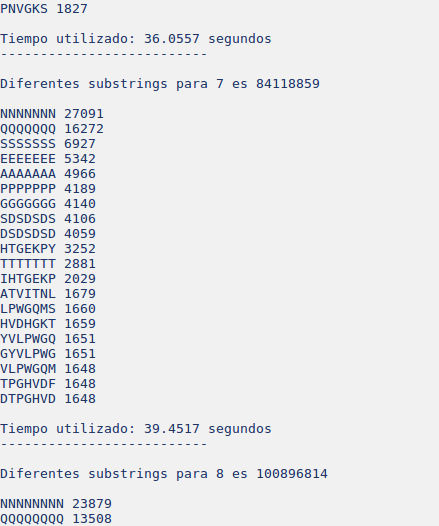
\includegraphics[width=0.5\textwidth]{./images/formatosalidaswissprot.png}
    \caption{Extracto del archivo de salida ``resultados\_k1to50.txt''}
\end{figure}

Como se puede apreciar en la imagen, se han guardado las cantidades de diferentes substrings obtenidos para cada $k$ (en la imagen se muestra para $k = 7$), los 20 residuos que más repiten con su respectiva cantidad de repeticiones encontradas y el tiempo en recorrer los arreglos para determinado $k$. Las líneas salteadas indican el cambio hacia el siguiente $k$ (para la imagen es $k=8$) nuevamente mostrando los diferentes substrings encontrados y los 20 residuos que más se repiten. Este proceso inicia con $k=1$ hasta llegar a $k=50$.

\subsection{Implementación solución para base de datos UniProt-TrEMBL}
%archivo implementacion
\chapter{Resultados y análisis}

Aquí se mostrarán los resultados que se obtuvieron con los algoritmos mencionados en la sección anterior. Haciendo un pequeño recuento, los \textit{datasets} usados son archivos que utilizan un formato \textbf{.fasta} y son los siguientes:

\begin{table}[h]
\centering
\begin{tabular}{|l|c|c|c|}
\hline
\multicolumn{1}{|c|}{\textbf{Archivo}} & \textbf{Proteínas} & \textbf{Tamaño (MB)} & \textbf{Tamaño cadena (MB)} \\ \hline
Base de datos SwissProt    & 555.426                & 268,3                & 199,5              \\
Base de datos TrEMBL        & 89.396.316              & 40.900 (aprox.)       & 30.200 (aprox.)     \\
Base de datos EROP-Moscow        & 14.785                 & 1,5                  & 0,3526                \\
Proteínas humanas     & 86.298                 & 47,2                 & 38,2               \\ \hline
\end{tabular}
\caption{\textit{Datasets} utilizados para la obtención de resultados}
\label{tb:labelr1}
\end{table} 

\section{Sistema utilizado y método de experimentación}

El trabajo se realizó en un ordenador \textit{Acer Aspire ES14}, no obstante las implementaciones se ejecutaron en un servidor prestado para la ocasión por la Universidad. Los datos relevantes a esta máquina se aprecian en la \textbf{Tabla 4.2}.

Los códigos fueron realizados en C++, mediante el uso del entorno de desarrollo integrado (IDE) ``Code::Blocks'' \cite{codeblocks}. Al momento de ejecutar las implementaciones todo fue realizado en el terminal con comandos básicos.

Los resultados obtenidos se guardaron en archivos .txt, y se mostrarán en la siguiente sección.

\newpage

\begin{table}[h]
\centering
\begin{tabular}{|c|c|}
\hline
\textbf{Componente}     & \textbf{Descripción}                         \\ \hline
Nombre CPU              & Intel(R) Xeon(R) CPU E5-2630 @2.30GHz        \\
CPU (s)                 & 12                                           \\
Caché (capacidad)       & 15 MB                                        \\
Memoria RAM (capacidad) & 60 GB                                        \\
Sistema Operativo       & Ubuntu Server 16.04 (Linux versión 4.4.0-51) \\ \hline
\end{tabular}
\caption{Especificaciones del sistema utilizado}
\label{tb:labelr2}
\end{table}

\section{Resultados obtenidos}

\subsection{Tiempos obtenidos}

Aquí se adjuntan las tablas con los tiempos logrados con las ejecuciones de los algoritmos con las 2 implementaciones explicadas en el capítulo anterior. Siguiendo este esquema se mostrarán en una tabla los tiempos obtenidos utilizando el algoritmo ``SwissProt'' (primera implementación explicada en el capítulo anterior relativa a alojar el arreglo de sufijos y el arreglo LCP en memoria RAM directamente) y en otra tabla los tiempos utilizando el algoritmo ``TrEMBL'' (capítulo anterior, segunda implementación relacionada a la obtención de los arreglos en memoria externa) ajustando la cantidad de memoria RAM usada a 20 GB para tanto el arreglo de sufijos como el arreglo LCP en memoria externa. 

En esta primera tabla se mostrará el tiempo en construir el arreglo de sufijos, el arreglo LCP y el tiempo empleado para obtener los diferentes substrings y los residuos que más se repiten con $k$ entre 1 a 50 (``Tiempo programa'').

\begin{table}[h]
\centering
\begin{tabular}{|l|c|c|c|}
\hline
\multicolumn{1}{|c|}{\textbf{Archivo}}  & \textbf{Tiempo SA (s)} & \textbf{Tiempo LCP (s)} & \textbf{Tiempo programa (s)} \\ \hline
SwissProt         & 2.637,18                & 35,09                   & 2.758,82                         \\
TrEMBL            & -                & -                &        -                  \\
EROP-Moscow       & 1,92                   & 0,03                    & 3,58                         \\
Proteínas humanas & 422,49                 & 9,06                    & 3,78 (k=1)                         \\ \hline
\end{tabular}
\caption{Tiempos de las implementaciones realizadas con los 4 \textit{datasets} utilizando el algoritmo ``SwissProt''}
\label{tb:labelr3}
\end{table}

Observando los tiempos del Tabla \ref{tb:labelr3} se aprecia que es mucho más rápido obtener el arreglo LCP que el el \textit{suffix array} para los casos analizados ya que la implementación del arreglo de sufijos considera ordenar los primeros \textit{p} sufijos (donde \textit{p} aumenta de manera exponencial en la iteración) y ese paso requiere tiempo, mientras que el arreglo LCP usa el arreglo de sufijos recién creado y la cadena para crear esta nueva estructura, y eso corresponde a analizar los elementos consecutivos del arreglo de sufijos respectivo (ver Tabla \ref{tb:labelr3}). Para este algoritmo no se pudo obtener los resultados con el archivo de ``TrEMBL'' ya que la cadena formada tenía un tamaño de 30 GB, con lo cual \textbf{ocupaba el 50\% de la capacidad disponible de la memoria RAM en el servidor}, en consecuencia generar 2 arreglos con la memoria RAM restante en base a este algoritmo no fue posible (problema tipo \texttt{std::bad\_alloc} en C++). 

\begin{table}[h]
\centering
\begin{tabular}{|l|c|c|c|c|}
\hline
\multicolumn{1}{|c|}{\textbf{Archivo (EM)}}  & \textbf{\begin{tabular}[c]{@{}c@{}}Tiempo\\SA (s)\end{tabular}} & \textbf{\begin{tabular}[c]{@{}c@{}}Tiempo\\LCP (s)\end{tabular}} & \textbf{\begin{tabular}[c]{@{}c@{}}Tiempo guardado\\elementos (s)\end{tabular}} & \textbf{\begin{tabular}[c]{@{}c@{}}Tiempo\\programa (s)\end{tabular}}\\ \hline
SwissProt         &  17,98               &  57,23                   &  59,39  &   4.533,09                        \\
TrEMBL            &  7.981,08               & 10.785,03                & 7.722,16       &  8,5 días                      \\
EROP-Moscow       & 0,23                   & 0,19             &   0,11  &    7,07                  \\
Proteínas humanas & 4,10                 & 9,40                    &  9,81        &  11,02              \\ \hline
\end{tabular}
\caption{Tiempos de las implementaciones realizadas con los 4 \textit{datasets} utilizando el algoritmo ``TrEMBL'' (EM = \textit{External Memory})}
\label{tb:labelr4}
\end{table}

Con respecto a los tiempos obtenidos en el Tabla \ref{tb:labelr4} se aprecia que la proporción entre tiempos de construcción de los arreglos LCP/SA son muy similares entre sí, a pesar de que el arreglo LCP se obtiene directamente del arreglo de sufijos recién obtenido. El motivo principal radica en que al aplicar los métodos de ``memoria externa'' (\textit{external memory}) se aplica la complejidad de I/O (entrada/salida, lecturas y escrituras en un archivo) y eso contribuye a \textbf{un aumento significativo de los tiempos en la obtención del arreglo LCP} (ver Tabla \ref{tb:labelr5}). Por otro lado también al Tabla \ref{tb:labelr4} se agrega la columna de ``Tiempo guardado elementos'' el cual es el tiempo que toma guardar los elementos de ambos arreglos en un archivo .txt para utilizarlos en el programa principal.

\begin{table}[h]
\centering
\begin{tabular}{|l|c|c|}
\hline
\multicolumn{1}{|c|}{\textbf{\begin{tabular}[c]{@{}c@{}}Proporción tiempos\\ LCP/SA\end{tabular}}} & \textbf{\begin{tabular}[c]{@{}c@{}}Algoritmo\\ SwissProt (\%)\end{tabular}} & \textbf{\begin{tabular}[c]{@{}c@{}}Algoritmo\\ TrEMBL (\%)\end{tabular}} \\ \hline
SwissProt            & 1,33       &   318,29                         \\
TrEMBL               & -          &   135,13                         \\
EROP-Moscow          & 1,56       &   82,60                          \\
Proteínas humanas    & 2,14       &   299,26                         \\ \hline
\end{tabular}
\caption{Relación entre tiempos de obtención del arreglo de sufijos y el arreglo LCP para los 2 algoritmos}
\label{tb:labelr5}
\end{table}

Apreciando la cantidad de memoria RAM asignada (20 GB), para SwissProt, EROP-Moscow y Proteínas humanas solamente es necesario un bloque de texto, ya que la capacidad de RAM es mucho más grande que los archivos mencionados, mientras que para el archivo de ``TrEMBL'' ya es necesario particionar el texto en bloques donde se obtienen arreglos de sufijos parciales (\textit{partial suffix arrays}) y de esa forma proseguir con la combinación (\textit{merging phase}) de estos arreglos para obtener el arreglo de sufijos y el arreglo LCP definitivo.

Comparando datos entre los Tablas \ref{tb:labelr3} y \ref{tb:labelr4}, se tiene que con motivos de comodidad es más sencillo trabajar estos archivos con el algoritmo ``SwissProt'' ya que no se ocupa complejidad I/O a la hora de construir los arreglos, no obstante el utilizar el algoritmo ``TrEMBL'' usa complejidad I/O y requiere más espacio en el disco duro, a costa de optimizar el tiempo de construcción de los arreglos. Otro punto relevante en este caso son los tiempos de ejecución del programa principal. Para ambos algoritmos la obtención de los diferentes substrings para cada $k$ y aquellos residuos que más se repiten sigue el mismo procedimiento con la importante diferencia que para el algoritmo ``TrEMBL'' los valores de los arreglos \textbf{se guardan en un archivo auxiliar en vez de un vector en memoria interna}, por lo tanto acceder a estos números requiere una mayor cantidad de tiempo de procesamiento.  

A nivel general la suma de los tiempos totales de ejecución de los algoritmos se presenta en el siguiente Tabla:


\begin{table}[h]
\centering
\begin{tabular}{|l|c|c|}
\hline
\multicolumn{1}{|c|}{\textbf{Archivo}} & \textbf{\begin{tabular}[c]{@{}c@{}}Algoritmo\\ SwissProt (s)\end{tabular}} & \textbf{\begin{tabular}[c]{@{}c@{}}Algoritmo\\TrEMBL (s)\end{tabular}} \\ \hline
SwissProt            & 5.431,09       &   4.667,69                         \\
TrEMBL               & -          &   8,8 días                         \\
EROP-Moscow          & 9,11       &   7,6                          \\
Proteínas humanas    & 435,33       &   34,33                         \\ \hline
\end{tabular}
\caption{Tiempos totales comparando entre los 2 algoritmos utilizados}
\label{tb:labelr14}
\end{table}

En todos los casos (a excepción del archivo TrEMBL) se aprecia que los tiempos usando el algoritmo de memoria externa son mucho más rápidos que utilizando el algoritmo ``SwissProt'' ya que, como anteriomente se indicó, existe la correlación de optimización de tiempo y uso de mayor memoria RAM disponible en sacrificio de guardar elementos en disco duro.

\subsubsection{Tamaño elementos guardados en disco duro para algoritmo ``TrEMBL''}

Para el algoritmo de memoria externa, en el proceso de construcción se guardaron archivos a partir de la cadena de strings de tamaño $n$ (el tamaño de la cadena para cada archivo está en el Tabla \ref{tb:labelr1}). Estos archivos son 4:

\begin{enumerate}

\item Archivo de $5n$ bytes para alojar arreglo de sufijos (formato .sa).
\item Archivo de $5n$ bytes para alojar arreglo LCP (formato .lcp).
\item Archivo que guarda los valores accesibles para el arreglo de sufijos (formato .txt).
\item Archivo que guarda los valores accesibles para el arreglo LCP (formato .txt).

\end{enumerate}

Para los 2 primeros \textit{items} estos arreglos usan un formato especial de salida (.sa y .lcp) por lo mismo no es posible acceder a ellos de manera trivial (usando comandos \texttt{open} y \texttt{getline} en C++). Por consiguiente en el proceso de construcción de estos arreglos se guardaron estos valores por separado en un archivo .txt para poder usarlos en el programa principal y de esa manera obtener los datos.

\begin{figure}[h]
    \centering
    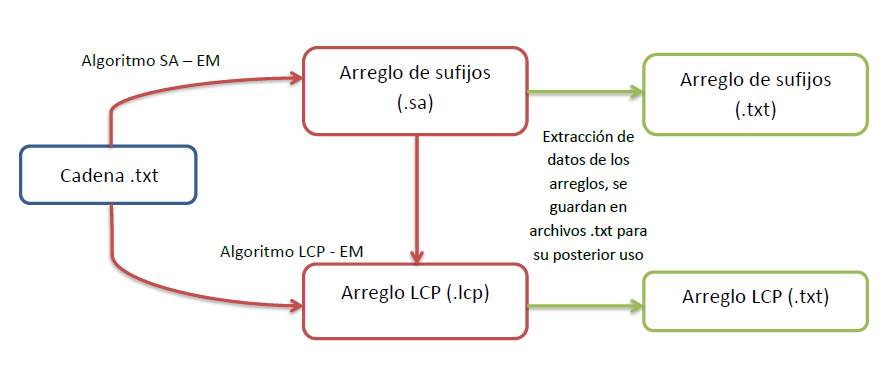
\includegraphics[width=1.0\textwidth]{./images/esquema_v1.PNG}
    \caption{Esquema sencillo de transformación de archivos para usarlos en el programa principal}
    \label{fig:imple1}
\end{figure}

Esto implica un gran uso de disco duro como punto en contra, más aún si se tiene que el archivo ``TrEMBL'' es muy pesado. Por lo tanto los pesos usados según cada archivo son los siguientes:

\begin{table}[h]
\centering
\begin{tabular}{|l|c|c|c|c|c|}
\hline
\multicolumn{1}{|c|}{\textbf{Archivo}} & \textbf{Archivo .sa} & \textbf{Archivo .lcp} & \textbf{\begin{tabular}[c]{@{}c@{}}Archivo\\accesible SA\end{tabular}} &  \textbf{\begin{tabular}[c]{@{}c@{}}Archivo\\accesible LCP\end{tabular}} & \textbf{Total}\\ \hline
SwissProt    & 997,5 MB                & 997,5 MB                 & 1,9 GB   & 524,8 MB & 4,41 GB\\
TrEMBL        & 151 GB              & 151 GB       & 351,3 GB   & 85,3 GB & 738,6 GB  \\
EROP-Moscow        & 1,8 MB                 & 1,8 MB                  & 2,4 MB         & 807,9 KB   &  6,80 MB \\
Proteínas humanas     & 191 MB                 & 191 MB                  & 332,6 MB       & 120,8 MB     &  835,4 MB  \\ \hline
\end{tabular}
\caption{Tamaños de archivos guardados en disco duro utilizando algoritmo ``TrEMBL''}
\label{tb:labelr15}
\end{table} 

En consecuencia los tamaños de los datos se hace gigantesco, en especial con el archivo que guarda los valores del arreglo SA. Recordar que los elementos que componen un arreglo de sufijos son todos números diferentes por ende al ir guardando números más grandes el peso requirido se va haciendo más alto; no obstante el arreglo LCP sí admite valores repetidos.\\
Así pues el usar este algoritmo de memoria externa implica un importante uso de la capacidad del disco duro, sin embargo en computadores actuales es factible guardar tamaña cantidad de peso, lo cual se mantendría si incluso se desea aumentar la capacidad de memoria RAM disponible para construir los arreglos en memoria externa, descendiendo los tiempos de obtención de estos archivos; aunque es difícil encontrar ordenadores con una memoria RAM superior a 20 GB con excepción de servidores de alta capacidad. 

\subsection{Diferentes substrings entre $k = 1$ hasta $k = 10$}

Los resultados obtenidos tomaron un rango de $k$ que va entre 1 hasta 50. En esta subsección se mostrarán los 10 primeros valores de $k$ (desde 1 hasta 10) ya que son los valores más relevantes con respecto a información de péptidos y porcentaje de residuos encontrados (las tablas completas serán colocadas en la sección \textbf{Apéndice} si se desean identificar mayores detalles de los valores obtenidos).

Siguiendo la ``Tabla 1'' que aparece en \cite{searching} se mostrarán los diferentes substrings encontrados para cada uno de los 4 archivos analizados, comparando según corresponda entre los algoritmos utilizados.

\subsubsection{Archivo SwissProt}

Los resultados obtenidos utilizando el archivo de SwissProt son los siguientes:

\begin{table}[h]
\centering
    \begin{tabular}{| c  r  r  c  r  c |}
    \hline
   \textbf{\begin{tabular}[c]{@{}c@{}}Largo\\péptido ($N$)\end{tabular}} & \multicolumn{1}{c}{\textbf{\begin{tabular}[c]{@{}c@{}}N-péptidos\\posibles ($20^{N}$)\end{tabular}}} & \textbf{\begin{tabular}[c]{@{}c@{}}Encontrados\\``SwissProt''\end{tabular}} & \textbf{\begin{tabular}[c]{@{}c@{}}Porcentaje\\encontrado (\%)\end{tabular}} & \textbf{\begin{tabular}[c]{@{}c@{}}Encontrados\\``TrEMBL''\end{tabular}} & \textbf{\begin{tabular}[c]{@{}c@{}}Porcentaje\\encontrado (\%)\end{tabular}} \\ \hline
    1 & 20 & 20 & 100,00 & 20 & 100,00 \\ \hline
    2 & 400 & 400 & 100,00 & 400 & 100,00 \\ \hline
    3 & 8.000 & 8.000 & 100,00 & 8.000 & 100,00 \\ \hline
    4 & 160.000 & 159.999 & 99,99 & 159.998 & 99,99\\ \hline
    5 & 3.200.000 & 3.113.509 & 97,29 & 3.113.510 & 97,29\\ \hline
    6 & 64.000.000 & 32.921.109 & 51,43 & 32.921.095 & 51,43\\ \hline
    7 & 1.280.000.000 & 84.118.859 & 6,57  & 84.118.817 & 6,57\\ \hline
    8 & 25.600.000.000 & 100.896.814 & 0,39 & 100.896.768 & 0,39\\ \hline
    9 & 512.000.000.000 & 105.834.330 & 0,020  & 105.834.282 & 0,020  \\ \hline
    10 & \multicolumn{1}{c}{1,024$\times 10^{13}$} & 108.976.567 & 0,0010 & 108.976.518 & 0,0010 \\ \hline   
    \end{tabular}
    \caption{Resultados de diferentes substrings obtenidos con el archivo SwissProt}
    \label{tb:labelr6}
\end{table}

Es posible identificar que los todos los potenciales residuos hasta un tamaño $k=3$ existen en esta base de datos, consideración importante si se tiene que las proteínas que componen este archivo no supera los 600.000. A partir de allí a medida que $k$ asciende aparecen más péptidos pero no aumentan al mismo ritmo que los potenciales residuos, por tanto aparece el brusco descenso de porcentaje, a ello se le agrega que los diferentes substrings encontrados se atascan en los 100 millones de proteínas si $k$ sigue en aumento. Con $k=10$ o superior el porcentaje de péptidos diferentes encontrados en relación a los potenciales péptidos \textbf{se hace ínfimo}, a niveles millodecimales. Por esta razón que aunque se presenten diferentes valores de residuos encontrados con los 2 algoritmos, si se lleva eso a porcentaje para ambos casos es lo mismo.

\subsubsection{Archivo TrEMBL}

Acá solamente se obtuvieron resultados con el algoritmo ``TrEMBL'' por las razones explicadas anteriormente, estos resultados son los siguientes:

\begin{table}[h]
\centering
    \begin{tabular}{| c  r  r  c |}
    \hline
   \textbf{\begin{tabular}[c]{@{}c@{}}Largo\\péptido ($N$)\end{tabular}} & \textbf{\begin{tabular}[c]{@{}c@{}}N-péptidos\\posibles ($20^{N}$)\end{tabular}} & \textbf{\begin{tabular}[c]{@{}c@{}}Encontrados\\``TrEMBL''\end{tabular}} & \textbf{\begin{tabular}[c]{@{}c@{}}Porcentaje\\encontrado (\%)\end{tabular}} \\ \hline
   
   1 & 20 & 20 & 100,00 \\ \hline
   2 & 400 & 400 & 100,00 \\ \hline
   3 & 8.000 & 8.000 & 100,00 \\ \hline
   4 & 160.000 & 160.000 & 100,00  \\ \hline
   5 & 3.200.000 & 3.200.000 & 100,00  \\ \hline
   6 & 64.000.000 & 63.817.907 & 99,71  \\ \hline
   7 & 1.280.000.000 & 1.024.659.629 & 80,05 \\ \hline
   8 & 25.600.000.000 & 5.743.538.889 & 22,43 \\ \hline
   9 & 512.000.000.000 & 10.114.868.387 & 1,97  \\ \hline
   10 & \multicolumn{1}{c}{1,024$\times 10^{13}$} & 11.524.607.918 & 0,11  \\ \hline
    \end{tabular}
    \caption{Resultados de diferentes substrings obtenidos con el archivo TrEMBL}
    \label{tb:labelr7}
\end{table}

La base de datos ``TrEMBL'' tiene un total de prácticamente 90 millones de proteínas, casi 164 veces el total de proteínas del archivo ``SwissProt'', por lo tanto es esperable encontrar una mayor cantidad de diferentes residuos y un porcentaje mayor con respecto al universo completo de posibles péptidos a encontrar para determinado $k$. Pues bien, los resultados muestran que esa tendencia se cumple a cabalidad, porque en este archivo \textbf{se encontraron que existen todos los potenciales residuos desde los aminoácidos hasta los pentapéptidos (péptidos compuestos de 5 aminoácidos)}. Con residuos de mayor tamaño ($k=6$ en adelante) comienza a bajar el porcentaje de péptidos encontrados, y sucede el mismo fenómeno que con el archivo SwissProt, los residuos diferentes encontrados se estancan en los 11 mil millones y a pesar que siguen en aumento conforme el valor de $k$ se incrementa, no lleva el mismo ritmo que los potenciales residuos a encontrar, tanto es así que para los péptidos compuestos de 10 aminoácidos los residuos encontrados solamente conforman el 0.1\% del universo total de residuos posibles.

\subsubsection{Archivo EROP-Moscow}

Para este archivo los resultados que se obtuvieron con ambos algoritmos son los siguientes:

\newpage
 
\begin{table}[h]
\centering
    \begin{tabular}{| c  r  r  c  r  c |}
    \hline
   \textbf{\begin{tabular}[c]{@{}c@{}}Largo\\péptido ($N$)\end{tabular}} & \textbf{\begin{tabular}[c]{@{}c@{}}N-péptidos\\posibles ($20^{N}$)\end{tabular}} & \textbf{\begin{tabular}[c]{@{}c@{}}Encontrados\\``SwissProt''\end{tabular}} & \textbf{\begin{tabular}[c]{@{}c@{}}Porcentaje\\encontrado (\%)\end{tabular}} & \textbf{\begin{tabular}[c]{@{}c@{}}Encontrados\\``TrEMBL''\end{tabular}} & \textbf{\begin{tabular}[c]{@{}c@{}}Porcentaje\\encontrado (\%)\end{tabular}} \\ \hline
    1 & 20 & 20 & 100,00 & 20 & 100,00 \\ \hline
    2 & 400 & 400 & 100,00 & 400 & 100,00 \\ \hline
    3 & 8.000 & 7.907 & 98,83 & 7.907 & 98,83 \\ \hline
    4 & 160.000 & 69.218 & 43,26 & 69.219 & 43,26 \\ \hline
    5 & 3.200.000 & 116.454 & 3,63 & 116.457 & 3,63 \\ \hline
    6 & 64.000.000 & 125.036 & 0,19 & 125.039 & 0,19 \\ \hline
    7 & 1.280.000.000 & 125.750 & 0,0098  & 125.752 & 0,0098 \\ \hline
    8 & 25.600.000.000 & 124.054 & 4,84$\times 10^{-4}$ & 124.055 & 4,84$\times 10^{-4}$\\ \hline
    9 & 512.000.000.000 & 121.103 & 2,36$\times 10^{-5}$  & 121.103 & 2,36$\times 10^{-5}$  \\ \hline
    10 & \multicolumn{1}{c}{1,024$\times 10^{13}$} & 117.457 & 1,14$\times 10^{-6}$ & 117.457 & 1,14$\times 10^{-6}$ \\ \hline   
    \end{tabular}
    \caption{Resultados de diferentes substrings obtenidos con el archivo EROP-Moscow}
    \label{tb:labelr8}
\end{table}

La base de datos EROP-Moscow se compone de 14.785 oligopéptidos cuyos tamaños varían entre 2 a 50 aminoácidos, por lo mismo se hace mucho más complejo encontrar un vasto conjunto de diferentes residuos para cada $k$. No obstante se encuentran \textbf{todos los posibles aminoácidos y dipéptidos existentes}, y con residuos de tamaño $k=3$ en adelante el porcentaje de péptidos encontrados se hace muy pequeño, lo cual es lógico ya que para tal cantidad de péptidos en este archivo es muy difícil obtener una mayor cantidad de diferentes péptidos. Este valor se estanca hasta los 125000 aproximadamente, y a partir de los residuos de tamaño $k=8$ el valor disminuye. Una explicación aparente para esto es que existen muchos péptidos compuestos de 5 aminoácidos o menos, por lo mismo para buscar péptidos con una magnitud de más de 5 aminoácidos son pocos los oligopéptidos del conjunto completo que cumplen la condición anteriormente mencionada, que se hace más notoria inclusive aumenta el valor de $k$. Por ejemplo en el caso de la búsqueda de residuos de tamaño $k=50$ se obtuvieron 116 elementos, que son 116 péptidos compuestos de 50 aminoácidos encontrados en la base de datos de EROP-Moscow sin elementos prohibidos.

\subsubsection{Archivo Proteínas Humanas}

Para este archivo solo se obtuvieron los diferentes substrings para $k=1$ y los resultados son los siguientes:

\begin{table}[h]
\centering
    \begin{tabular}{| c  c  c  c  c  c |}
    \hline
   \textbf{\begin{tabular}[c]{@{}c@{}}Largo\\péptido ($N$)\end{tabular}} & \textbf{\begin{tabular}[c]{@{}c@{}}N-péptidos\\posibles ($20^{N}$)\end{tabular}} & \textbf{\begin{tabular}[c]{@{}c@{}}Encontrados\\``SwissProt''\end{tabular}} & \textbf{\begin{tabular}[c]{@{}c@{}}Porcentaje\\encontrado (\%)\end{tabular}} & \textbf{\begin{tabular}[c]{@{}c@{}}Encontrados\\``TrEMBL''\end{tabular}} & \textbf{\begin{tabular}[c]{@{}c@{}}Porcentaje\\encontrado (\%)\end{tabular}} \\ \hline
    1 & 20 & 20 & 100,00 & 20 & 100,00 \\ \hline  
    \end{tabular}
    \caption{Resultados de diferentes substrings obtenidos con el archivo Proteínas Humanas}
    \label{tb:labelr9}
\end{table}

En lo que corresponde a las proteínas que existen en el ser humano se puede rescatar que utilizando ambos algoritmos \textbf{se obtienen los 20 aminoácidos buscados (100\%)}. Como para este archivo se está trabajando con solo un $k=1$, se realizará un mayor análisis biológico en la subsección siguiente, para este caso, aquellos aminoácidos que más se repiten.

\subsubsection{Diferencias entre resultados obtenidos utilizando el algoritmo ``SwissProt'' y el algoritmo ``TrEMBL''}

En los Tablas mostrados anteriormente, para los archivos SwissProt y EROP-Moscow se identifica que según un determinado $k$ varios de los diferentes substrings encontrados entrega diferentes valores usando ambos algoritmos ($k=4$ o superior para base de datos SwissProt y varios $k$ para EROP-Moscow). ¿Esto implica que uno de los algoritmos utilizados está incorrecto? ¿O acaso los 2 algoritmos están incorrectos?\\
Cuando se comenzó a trabajar con este tipo de cadenas, destacados investigadores como Gonzalo Navarro \cite{navarro2016} han expuesto que utilizar datos compactos es lo más conveniente, porque el procesamiento de texto es más rápido y expedito de comprender. Dentro de esto grupo enorme de estructuras que trabajan con datos tipo cadena se eligió el arreglo de sufijos y el arreglo LCP.\\
Pues bien, para llevar a tierra todo lo investigado en información es importante obtener \textbf{datos concretos de experimentación}, que se han mostrado en cada uno de los Tablas anteriores. Por consiguiente al experimentar con estos algoritmos es bastante factible obtener varias diferencias de resultados obtenidos, que según apreciando el porcentaje de péptidos encontrados, son los mismos, a tal punto que se necesita \textbf{llegar a la tercera o cuarta cifra significativa para recíen encontrar diferencias} entre estos porcentajes.

Observando desde el lado de la implementación realizada, los arreglos obtenidos se aplican según esquemas establecidos por investigadores, para el lado del algoritmo desarrollado por Kasai \cite{kasai} como para los algoritmos de memoria externa (\cite{sascan}, \cite{emsparse}), por ende se hallan diferencias de implementación los cuales definan estas diferencias de resultados. Otra cosa importante es que las cadenas usadas son tan grandes que ocupan tamaños cercanos a los 200 millones de caracteres, a los cuales se le revisa su posición y sufijo al que pertenece para poder extraer aquel residuo con su número (cantidad de veces que aparece en la base de datos) y guardarlo en el \textit{priority queue}, por ende el procedimiento realizado también puede dar con estas diferencias que a la larga son muy pequeñas por los porcentajes que se obtuvieron.

Para intentar corroborar se podría usar una opción poco ortodoxa, que sería obtener los diferentes substrings para cada archivo usando un algoritmo de fuerza bruta, pero realizar esto no es recomendable ya que a nivel de tiempo es el algoritmo más malo que se puede hallar, si se entrega como \textit{input} el archivo de TrEMBL a este algoritmo demoraría meses en obtener los resultados solicitados.

Tomando en consideración esto, se procederá a resumir en un gráfico de Porcentaje v/s $k$ cómo evoluciona el porcentajes de péptidos encontrados según los péptidos posibles a encontrar. Como para cada archivo los porcentajes obtenidos con cada algoritmo utilizado son los mismos se mostrarán 4 líneas, cada una según el archivo al que pertenezca:

\newpage

\begin{figure}[h]
    \centering
    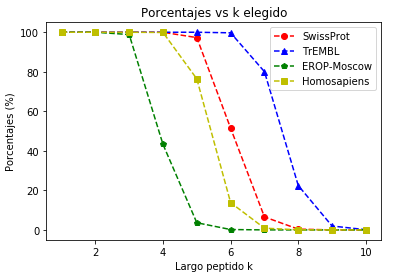
\includegraphics[width=0.6\textwidth]{./images/grafico1v1.png}
    \caption{Gráfico que muestra los porcentajes de residuos encontrados según el largo de péptido $k$ para los 4 archivos}
    \label{fig:imple2}
\end{figure}

Observando el gráfico, se aprecia que los valores obtenidos en los porcentajes dependen \textbf{directamente de la cantidad de proteínas} que contenga la base de datos (la relación de tamaños de los archivos sigue el siguiente patrón: TrEBML $>$ SwissProt $>$ Homosapiens $>$ EROP-Moscow), es decir, si se tienen más proteínas será mayor la diversidad de residuos a encontrar. Hasta $k=3$ es posible identificar en todos los archivos que poseen casi todos los residuos posibles, a partir de ese punto comienzan a bajar las probabilidades de localizar un mayor porcentaje de substrings de tamaño $k$. En todos los casos esta bajada en probabilidades es brusca, tomando en cuenta que los posibles péptidos de tamaño $k$ se rigen según la fórmula $20^{k}$. Al contener esta fórmula como base al 20, el salto exponencial que implica ir de $k$ a $k+1$ es muy fuerte, tanto es así que por ejemplo el archivo TrEMBL, a pesar de ser 164 veces más grande que el archivo SwissProt, abarca solamente un 20\% de los posibles residuos que se pueden encontrar de tamaño 8 ($20^{8} = 25.600.000.000$), mientras que SwissProt abarca menos del 0.5\% de residuos posibles para este $k$.\\
Para $k=10$ los porcentajes de substrings encontrados para los 4 archivos es prácticamente 0, por esa razón es que se decidió mostrar los el comportamiento de los diferentes substrings localizados hasta un tamaño igual a 10, para $k$ mayores a este valor los resultados de los porcentajes serían muy pequeños, prácticamente a escalas atómicas. 

\subsection{Substrings de determinado $k$ que más se repiten}

Ahora se mostrarán los substrings de tamaño $k$ que más se repiten en los 4 \textit{datasets} trabajados. Para cada $k$ se obtuvieron los 20 residuos que más se repiten, no obstante por motivos de espacio se mostrarán en esta sección los 5 substrings que más se repiten variando $k$ entre 1 hasta 10 (hasta 8 para SwissProt por motivos de espacios) como se hizo en el análisis anterior (las tablas completas con los 3 substrings que más se repiten variando $k$ entre 1 hasta 50 serán colocadas en la sección \textbf{Apéndice}, se consideraron los 3 primeros por motivos de espacio). Primero se presentarán las tablas obtenidas y luego se le hará un análisis a estos resultados.

\subsubsection{Archivo SwissProt}

\begin{table}[h]
\centering
\begin{tabular}{|c|r|r|c|c|r|r|}
\cline{1-3} \cline{5-7}
\textbf{k} & \multicolumn{1}{c|}{\textbf{\begin{tabular}[c]{@{}c@{}}Algoritmo \\ SwissProt\end{tabular}}}                          & \multicolumn{1}{c|}{\textbf{\begin{tabular}[c]{@{}c@{}}Algoritmo\\ TrEMBL\end{tabular}}}                              & \multicolumn{1}{l|}{} & \textbf{k} & \multicolumn{1}{c|}{\textbf{\begin{tabular}[c]{@{}c@{}}Algoritmo\\ SwissProt\end{tabular}}}                                                        & \multicolumn{1}{c|}{\textbf{\begin{tabular}[c]{@{}c@{}}Algoritmo\\ TrEMBL\end{tabular}}}                                                           \\ \cline{1-3} \cline{5-7} 
1  & \begin{tabular}[c]{@{}r@{}}L - 19.206.802\\ A - 16.435.230\\ G - 14.086.821\\ V - 13.664.059\\ E - 13.406.543\end{tabular}      & \begin{tabular}[c]{@{}r@{}}L - 19.206.802\\ A - 16.435.229\\ G - 14.086.821\\ V - 13.664.059\\ E - 13.406.543\end{tabular}      &                       & 5  & \begin{tabular}[c]{@{}r@{}}NNNNN - 36.977\\ QQQQQ - 26.232\\ SSSSS - 17.652\\ AAAAA - 17.020\\ EEEEE - 13.572\end{tabular} & \begin{tabular}[c]{@{}r@{}}NNNNN - 36.977\\ QQQQQ - 26.232\\ SSSSS - 17.652\\ AAAAA - 17.020\\ EEEEE - 13.572\end{tabular} \\ \cline{1-3} \cline{5-7} 
2  & \begin{tabular}[c]{@{}r@{}}LL - 1.886.886\\ AA - 1.714.607\\ AL - 1.683.204\\ LA - 1.673.336\\ LS - 1.337.091\end{tabular}      & \begin{tabular}[c]{@{}r@{}}LL - 1.886.886\\ AA - 1.714.607\\ AL - 1.683.204\\ LA - 1.673.336\\ LS - 1.337.091\end{tabular}      &                       & 6  & \begin{tabular}[c]{@{}r@{}}NNNNNN - 31.269\\ QQQQQQ - 20.197\\ SSSSSS - 10.379\\ AAAAAA - 8.392\\ EEEEEE -   8.077\end{tabular}                       & \begin{tabular}[c]{@{}r@{}}NNNNNN - 31.269\\ QQQQQQ - 20.197\\ SSSSSS - 10.379\\ AAAAAA -   8.392\\ EEEEEE -   8.077\end{tabular}                                     \\ \cline{1-3} \cline{5-7} 
3 & \begin{tabular}[c]{@{}r@{}}AAA - 232.439\\ ALA - 185.750\\ LLL - 180.299\\ LAA - 179.704\\ AAL - 177.751\end{tabular}      & \begin{tabular}[c]{@{}r@{}}AAA - 232.439\\ ALA - 185.750\\ LLL - 180.299\\ LAA - 179.704\\ AAL - 177.751\end{tabular}      &                       & 7  & \begin{tabular}[c]{@{}r@{}}NNNNNNN - 27.091\\ QQQQQQQ - 16.272\\ SSSSSSS -   6.927\\ EEEEEEE -   5.342\\ AAAAAAA -   4.966\end{tabular}                 & \begin{tabular}[c]{@{}r@{}}NNNNNNN - 27.091\\ QQQQQQQ - 16.272\\ SSSSSSS -   6.927\\ EEEEEEE -   5.342\\ AAAAAAA -   4.966\end{tabular}              \\ \cline{1-3} \cline{5-7} 
4   & \begin{tabular}[c]{@{}r@{}}AAAA - 47.284\\ NNNN - 46.321\\ SSSS - 39.923\\ QQQQ - 36.956\\ EEEE - 29.213\end{tabular}      & \begin{tabular}[c]{@{}r@{}}AAAA - 47.284\\ NNNN - 46.321\\ SSSS - 39.923\\ QQQQ - 36.956\\ EEEE - 29.213\end{tabular}      &                       & 8 & \begin{tabular}[c]{@{}r@{}}NNNNNNNN - 23.879\\ QQQQQQQQ - 13.508\\ SSSSSSSS -   5.006\\ SDSDSDSD -   3.905\\ DSDSDSDS -   3.875\end{tabular}            & \begin{tabular}[c]{@{}r@{}}NNNNNNNN - 23.879\\ QQQQQQQQ - 13.508\\ SSSSSSSS -   5.006\\ SDSDSDSD -   3.905\\ DSDSDSDS -   3.875\end{tabular}       \\ \cline{1-3} \cline{5-7} 
\end{tabular}
\caption{Residuos más repetidos usando $k$ entre 1 hasta 8 para el archivo SwissProt}
\label{tb:labelr10}
\end{table}

Apreciando bien se identifica que para los 2 algoritmos los resultados obtenidos son los mismos, por otra parte es que las cantidades de los valores más repetidos van disminuyendo muy rápidamente (para $k = 1$ los valores repetidos rondan las 10 millones de repeticiones y para $k = 2$ rondan solamente el millón de repeticiones). Otro punto relevante es que muchas repeticiones son residuos compuestos solamente por un aminoácido.

\newpage

\subsubsection{Archivo TrEMBL}

\begin{table}[h]
\centering
\begin{tabular}{|c|r|c|c|r|}
\cline{1-2} \cline{4-5}
\textbf{k} & \multicolumn{1}{c|}{\textbf{\begin{tabular}[c]{@{}c@{}}Algoritmo \\ TrEMBL\end{tabular}}}   & \multicolumn{1}{l|}{} & \textbf{k} & \multicolumn{1}{c|}{\textbf{\begin{tabular}[c]{@{}c@{}}Algoritmo\\ TrEMBL\end{tabular}}}   \\ \cline{1-2} \cline{4-5} 
1  & \begin{tabular}[c]{@{}r@{}}L - 2.966.351.173\\ A - 2.715.689.443\\ G - 2.175.272.504\\ V - 2.065.665.475\\ S - 2.030.276.782\end{tabular} &  & 6  & \begin{tabular}[c]{@{}r@{}}QQQQQQ - 2.355.101\\ AAAAAA - 1.496.140\\ SSSSSS - 1.411.002\\ GGGGGG - 898.024\\ NNNNNN - 861.564\end{tabular}                        \\ \cline{1-2} \cline{4-5} 
2  & \begin{tabular}[c]{@{}r@{}}AA - 313.028.096\\ LL - 306.619.288\\ LA - 285.314.569\\ AL - 281.904.750\\ AG - 212.968.976\end{tabular}       &                       & 7  & \begin{tabular}[c]{@{}r@{}}QQQQQQQ - 1.798.936\\ SSSSSSS - 922.266\\ AAAAAAA - 880.843\\ WTVYPPL - 815.253\\ GWTVYPP - 814.768\end{tabular}             \\ \cline{1-2} \cline{4-5}  
3 & \begin{tabular}[c]{@{}r@{}}AAA - 45.269.369\\ LAA - 34.321.839\\ ALA - 34.225.481\\ AAL - 33.850.558\\ LLL - 32.856.884\end{tabular}     &                       & 8 & \begin{tabular}[c]{@{}r@{}}QQQQQQQQ - 1.408.675\\ GWTVYPPL - 813.630\\ TGWTVYPP - 798.282\\ GTGWTVYP - 798.215\\ MIFFMVMP - 771.616\end{tabular}            \\ \cline{1-2} \cline{4-5} 
4   & \begin{tabular}[c]{@{}r@{}}AAAA - 9.197.193\\ SSSS - 5.754.913\\ ALAA - 5.176.104\\ LLLL - 5.111.818\\ AALA - 5.085.892\end{tabular}   &                       & 9  & \begin{tabular}[c]{@{}r@{}}QQQQQQQQQ - 1.124.827\\ GTGWTVYPP - 797.778\\ TGWTVYPPL - 797.178\\ LLLLSLPVL - 756.549\\ LLLSLPVLA - 751.235\end{tabular}      \\ \cline{1-2} \cline{4-5} 
5  & \begin{tabular}[c]{@{}r@{}}QQQQQ - 3.210.070\\ AAAAA - 3.108.174\\ SSSSS - 2.473.516\\ GGGGG - 1.679.232\\ PPPPP - 1.473.476\end{tabular} &                       & 10 & \begin{tabular}[c]{@{}r@{}}QQQQQQQQQQ - 911.438\\ GTGWTVYPPL - 796.679\\ LLLLSLPVLA - 749.816\\ PDMAFPRMNN - 667.479\\ FPRMNNMSFW - 661.041\end{tabular}  \\ \cline{1-2} \cline{4-5} 
\end{tabular}
\caption{Residuos más repetidos usando $k$ entre 1 hasta 10 para el archivo TrEMBL}
\label{tb:labelr11}
\end{table}

Acá solo se muestran los resultados con los algoritmos de memoria externa ya que con el algoritmo SwissProt no se pudo analizar esta base de datos (los motivos fueron explicados anteriormente).\\
Los péptidos más repetidos obtenidos para este archivo entregan resultados muy similares a los conseguidos con el archivo SwissProt con respecto a \textbf{los residuos}. Este fenómeno será explicado más adelante.

\newpage

\subsubsection{Archivo EROP-Moscow}

\begin{table}[h]
\centering
\begin{tabular}{|c|r|r|c|c|r|r|}
\cline{1-3} \cline{5-7}
\textbf{k} & \multicolumn{1}{c|}{\textbf{\begin{tabular}[c]{@{}c@{}}Algoritmo \\ SwissProt\end{tabular}}}                & \multicolumn{1}{c|}{\textbf{\begin{tabular}[c]{@{}c@{}}Algoritmo\\ TrEMBL\end{tabular}}}                    & \multicolumn{1}{l|}{} & \textbf{k} & \multicolumn{1}{c|}{\textbf{\begin{tabular}[c]{@{}c@{}}Algoritmo\\ SwissProt\end{tabular}}}                                     & \multicolumn{1}{c|}{\textbf{\begin{tabular}[c]{@{}c@{}}Algoritmo\\ TrEMBL\end{tabular}}}                                        \\ \cline{1-3} \cline{5-7} 
1                                                                      & \begin{tabular}[c]{@{}r@{}}G - 30.373\\ L - 23.867\\ K - 21.956\\ S - 21.486\\ C - 21.365\end{tabular}           & \begin{tabular}[c]{@{}r@{}}G - 30.373\\ L - 23.867\\ K - 21.956\\ S - 21.486\\ C - 21.365\end{tabular}           &                       & 6                                                                      & \begin{tabular}[c]{@{}r@{}}RRRRRR - 160\\ FDEIDR - 127\\ NFDEID - 114\\ CGLSGL - 98\\ GLSGLC - 94\end{tabular}                  & \begin{tabular}[c]{@{}r@{}}RRRRRR - 160\\ FDEIDR - 127\\ NFDEID - 114\\ CGLSGL - 98\\ GLSGLC - 94\end{tabular}                  \\ \cline{1-3} \cline{5-7} 
2                                                                      & \begin{tabular}[c]{@{}r@{}}GL - 3.307\\ RR - 2.904\\ GG - 2.872\\ GK - 2.558\\ AA - 2.493\end{tabular}           & \begin{tabular}[c]{@{}r@{}}GL - 3.307\\ RR - 2.904\\ GG - 2.872\\ GK - 2.558\\ AA - 2.493\end{tabular}           &                       & 7                                                                      & \begin{tabular}[c]{@{}r@{}}NFDEIDR - 102\\ CGLSGLC - 88\\ VCGLSGL - 79\\ MEHFRWG - 76\\ FDEIDRS - 72\end{tabular}               & \begin{tabular}[c]{@{}r@{}}NFDEIDR - 102\\ CGLSGLC - 88\\ VCGLSGL - 79\\ MEHFRWG - 76\\ FDEIDRS - 72\end{tabular}               \\ \cline{1-3} \cline{5-7} 
3                                                                      & \begin{tabular}[c]{@{}r@{}}RRR - 1.253\\ FGL - 483\\ GGG - 479\\ LSG - 469\\ AAK - 451\end{tabular}          & \begin{tabular}[c]{@{}r@{}}RRR - 1.253\\ FGL - 483\\ GGG - 479\\ LSG - 469\\ AAK - 451\end{tabular}          &                       & 8                                                                      & \begin{tabular}[c]{@{}r@{}}VCGLSGLC - 71\\ EHFRWGKP - 68\\ MEHFRWGK - 68\\ SMEHFRWG - 65\\ YSMEHFRW - 62\end{tabular}           & \begin{tabular}[c]{@{}r@{}}VCGLSGLC - 71\\ EHFRWGKP - 68\\ MEHFRWGK - 68\\ SMEHFRWG - 65\\ YSMEHFRW - 62\end{tabular}           \\ \cline{1-3} \cline{5-7} 
4                                                                      & \begin{tabular}[c]{@{}r@{}}RRRR - 712\\ GGGG - 183\\ GCSC - 172\\ CCSG - 167\\ LSGL - 162\end{tabular}      & \begin{tabular}[c]{@{}r@{}}RRRR - 712\\ GGGG - 183\\ GCSC - 172\\ CCSG - 167\\ LSGL - 162\end{tabular}      &                       & 9                                                                      & \begin{tabular}[c]{@{}r@{}}MEHFRWGKP - 68\\ SMEHFRWGK - 65\\ YSMEHFRWG - 61\\ EHFRWGKPV - 59\\ GGTCNTPGC - 59\end{tabular}      & \begin{tabular}[c]{@{}r@{}}MEHFRWGKP - 68\\ SMEHFRWGK - 65\\ YSMEHFRWG - 61\\ EHFRWGKPV - 59\\ GGTCNTPGC - 59\end{tabular}      \\ \cline{1-3} \cline{5-7} 
5                                                                      & \begin{tabular}[c]{@{}r@{}}RRRRR - 373\\ FDEID - 144\\ DEIDR - 139\\ CGLSG - 128\\ GGGGG - 121\end{tabular} & \begin{tabular}[c]{@{}r@{}}RRRRR - 373\\ FDEID - 144\\ DEIDR - 139\\ CGLSG - 128\\ GGGGG - 121\end{tabular} &                       & 10                                                                     & \begin{tabular}[c]{@{}r@{}}SMEHFRWGKP - 65\\ YSMEHFRWGK - 61\\ MEHFRWGKPV - 59\\ SYSMEHFRWG - 53\\ EHFRWGKPVG - 46\end{tabular} & \begin{tabular}[c]{@{}r@{}}SMEHFRWGKP - 65\\ YSMEHFRWGK - 61\\ MEHFRWGKPV - 59\\ SYSMEHFRWG - 53\\ EHFRWGKPVG - 46\end{tabular} \\ \cline{1-3} \cline{5-7} 
\end{tabular}
\caption{Residuos más repetidos usando $k$ entre 1 hasta 10 para el archivo EROP-Moscow}
\label{tb:labelr12}
\end{table}

Con este archivo ya es posible obtener los resultados con los 2 algoritmos sin problemas, además se aprecia que los valores obtenidos son los mismos para cada algoritmo utilizado.\\
Para esta base de datos los péptidos obtenidos distan de los encontrados en los archivos anteriores, de hecho no aparecen residuos compuestos por un solo aminoácido (a excepción de ``R'' y ``G''), lo que tiene relación con la \textbf{base de datos utilizada}. Al ser este un análisis más biológico, se tratará más adelante.

\subsubsection{Archivo Proteínas Humanas}

\begin{table}[h]
\centering
\begin{tabular}{|c|r|r|}
\cline{1-3}
\textbf{k} & \multicolumn{1}{c|}{\textbf{\begin{tabular}[c]{@{}c@{}}Algoritmo \\ SwissProt\end{tabular}}}                & \multicolumn{1}{c|}{\textbf{\begin{tabular}[c]{@{}c@{}}Algoritmo\\ TrEMBL\end{tabular}}}    \\ \cline{1-3}

1                                                                      & \begin{tabular}[c]{@{}r@{}}L - 3.979.937\\ S - 3.123.633\\ A - 2.631.167\\ E - 2.467.325\\ G - 2.448.081\\ P - 2.336.530\\ T - 2.248.068\\ V - 2.229.816\\ K - 2.082.746\\ R - 2.012.813\\ I - 1.863.090\\ D - 1.723.766\\ Q - 1.715.384\\ F - 1.448.281\\ N - 1.448.115\\ Y - 1.078.310\\ H - 997.696\\ M - 922.926\\ C - 805.709\\ W - 527.194\end{tabular} & \begin{tabular}[c]{@{}r@{}}L - 3.979.937\\ S - 3.123.633\\ A - 2.631.167\\ E - 2.467.325\\ G - 2.448.081\\ P - 2.336.530\\ T - 2.248.068\\ V - 2.229.816\\ K - 2.082.746\\ R - 2.012.813\\ I - 1.863.090\\ D - 1.723.766\\ Q - 1.715.384\\ F - 1.448.281\\ N - 1.448.115\\ Y - 1.078.310\\ H - 997.696\\ M - 922.926\\ C - 805.709\\ W - 527.194\end{tabular}           \\ \cline{1-3}

\end{tabular}
\caption{Residuos más repetidos usando $k = 1$ para el archivo Proteínas Humanas}
\label{tb:labelr13}
\end{table}


Al ser solamente $k=1$ a analizar para este archivo (se consideró eso ya que la finalidad era identificar a aquellos aminoácidos que más están presentes en el ser humano) se decide mostrar para ambos algoritmos la cantidad de veces que se repiten cada uno de los 20 aminoácidos.\\
Se puede identificar que los resultados obtenidos utilizando cualquiera de los 2 algoritmos es el mismo, lo cual entrega veracidad a los resultados logrados.

\subsubsection{Análisis de resultados (enfoque algorítmico)}

Los resultados conseguidos con los 2 algoritmos en esta sección son similares, por ende otorgan veracidad a la hora de definir que la estrategia de utilizar arreglos de sufijos y arreglos LCP era la indicada. Más importante aún, queda de manifiesto que la opción de uso de la estructura conocida como \textbf{\textit{priority queue}} es la correcta ya que permite guardar substrings enlazados con su respectivo valor para luego extraer aquellos residuos con más altos valores. Su utilización permitió identificar estos datos importantes y construir estas Tablas de información, por consiguiente parece ser la opción indicada a la hora de buscar ordenar números, strings u otro tipo de variables siguiendo un orden de jerarquía determinado con anterioridad.

\subsubsection{Análisis de resultados (enfoque biológico)}

Para realizar este análisis, al ser un ámbito fuera de la informática se solicitó ayuda y consejos del profesor Alexander Zamyatnin. Este análisis será realizado de manera muy superficial de manera que pueda ser entendido por el lector sin mayor conocimiento de la biología, una mayor profundización a esto será considerado trabajo futuro entre el profesor mencionado y el autor de esta memoria, y publicado en un escrito (\textit{paper}).
 
Recordando un poco, la estructura de un aminoácido sigue el siguiente formato:

\begin{figure}[h]
    \centering
    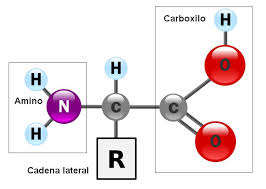
\includegraphics[width=0.4\textwidth]{./images/estructura2.jpeg}
    \caption{Estructura de un aminoácido, donde se identifica el grupo amino (izquierda), grupo carboxilo (derecha) y el grupo radical (R)}
    \label{fig:imple3}
\end{figure}

Con respecto a la frecuencia de los residuos de aminoácidos encontrados para la base de datos de UniProt (SwissProt, TrEMBL y Homosapiens), los aminoácidos L (Leucina), A (Alanina), G (Glicina), V (Valina) y E (Ácido Glutámico) son los más comunes debido a sus características físico-químicas, en especial para L, A y V, que son \textbf{residuos hidrofóbicos} (L es el residuo más hidrofóbico). Cuando se habla de aminoácidos hidrofóbicos \cite{quimicaaminoacidos}, su característica principal es que tienden a rechazar el ambiente acuoso (agua) y, por lo tanto, residen predominante dentro de las proteínas. Estos residuos se utilizan para la estabilización de la estructura global de muchas proteínas (en especial aquellas con más de 50 aminoácidos).\\
Por el contrario, los aminoácidos hidrofílicos tienden a interactuar con el ambiente acuoso, se encuentra ubicados en los sectores extremos de una cadena de polipéptidos y están implicados a menudo en la formación de enlaces de H para la unión entre aminoácidos.

En el caso de los ``oligopéptidos reguladores'' (base de datos de EROP-Moscow) los aminoácidos G, L, K (Lisina), S (Serina) y C (Cisteína) son los residuos más comunes. Estos oligopéptidos \cite{zamyatnin3} son moléculas flexibles que cambian su configuración física, poseen pocas interacciones moleculares y muy débiles (pocos residuos hidrofóbicos), tienen fuertes enlaces covalentes (enlaces entre elementos no metálicos de la Tabla Periódica de Elementos Químicos) intramoleculares entre los residuos C-C y participan en variadas interacciones electroestáticas.

En relación a las repeticiones encontradas de un solo aminoácido, muchas de los animoácidos pueden tener carácterísticas ácidas (pH bajo) como N (Aspargarina) o Q (Glutamina) los cuales buscan enlazarse con sus pares ya que poseen los grupos amino y carboxilo polarizados a nivel de carga eléctrica, y de esa forma producir un enlace entre aminoácidos.
%fin desarrollo

%archivo conclusiones
\chapter*{Conclusiones}
\addcontentsline{toc}{chapter}{Conclusiones}







\begin{thebibliography}{9}
\bibitem{latexcompanion} 
Michel Goossens, Frank Mittelbach, and Alexander Samarin. 
\textit{The \LaTeX\ Companion}. 
Addison-Wesley, Reading, Massachusetts, 1993.
 
\bibitem{einstein} 
Albert Einstein. 
\textit{Zur Elektrodynamik bewegter K{\"o}rper}. (German) 
[\textit{On the electrodynamics of moving bodies}]. 
Annalen der Physik, 322(10):891–921, 1905.
 
\bibitem{knuthwebsite} 
Knuth: Computers and Typesetting,
\\\texttt{http://www-cs-faculty.stanford.edu/\~{}uno/abcde.html}

\bibitem{bioinformatica} 
Rafael Lahoz-Beltrá.
\textit{BIOINFORMÁTICA, simulación, vida artificial e inteligencia artificial}. 
Ediciones Díaz de Santos S.A., Madrid, España, 2004.

\bibitem{searching} 
Bruce C. Orcutt, Winona C. Barker.
\textit{Searching the protein sequence database}.
National Biomedical Research Foundation, Georgetown University Medical Center,
Washington, D.C., \textit{Bulletin of Mathematical Biology}, 46(4):545-552, 1984.

\bibitem{array} 
Alexander A. Zamyatnin.
\textit{The Features of an Array of Natural Oligopeptides}.
Bakh Institute of Biochemistry, Russian Academy of Sciences, Moskow, Russia;
Departamento de Informática, Universidad Técnica Federico Santa María, Valparaíso, Chile,
\textit{Neurochemical Journal}, 10(4):249-257, 2016.

\bibitem{biomolecula} 
Wikipedia, Definición de biomolécula,
\\\texttt{https://es.wikipedia.org/wiki/Biomolécula}.

\bibitem{amino} 
Jan Koolman, Klaus-Heinrich Röhm
\textit{Bioquímica: Texto y Atlas}.
Editorial Médica Panamericana, Madrid, España;
Georg Thieme Verlag, Stuttgart, Germany, 2004.

\bibitem{zamyatnin1} 
A. A. Zamyatnin, 
\textit{Fragmentomics of Natural Peptide Structures}. 
Bach Institute of Biochemistry, Russian Academy of Sciences;  Universidad Técnica Federico Santa María, Departamento de Informática, Valparaíso, 2009, pp. 405-428.

\bibitem{zamyatnin2} 
A. A. Zamyatnin, 
\textit{Fragmentomics of Oligopeptides and Proteins}. 
Bach Institute of Biochemistry, Russian Academy of Sciences;  Universidad Técnica Federico Santa María, Departamento de Informática, Valparaíso, 2nd Asia-Pacific International Peptide Symposium, 2007.

\end{thebibliography}



%\bibliographystyle{plain}
\bibliography{bib/papers}


%\backmatter
%\cleardoublepage

\singlespacing
\cleardoublepage





\end{document}
